% Options for packages loaded elsewhere
\PassOptionsToPackage{unicode}{hyperref}
\PassOptionsToPackage{hyphens}{url}
%
\documentclass[
]{article}
\title{Projet ThreeME}
\author{}
\date{\vspace{-2.5em}}

\usepackage{amsmath,amssymb}
\usepackage{lmodern}
\usepackage{iftex}
\ifPDFTeX
  \usepackage[T1]{fontenc}
  \usepackage[utf8]{inputenc}
  \usepackage{textcomp} % provide euro and other symbols
\else % if luatex or xetex
  \usepackage{unicode-math}
  \defaultfontfeatures{Scale=MatchLowercase}
  \defaultfontfeatures[\rmfamily]{Ligatures=TeX,Scale=1}
\fi
% Use upquote if available, for straight quotes in verbatim environments
\IfFileExists{upquote.sty}{\usepackage{upquote}}{}
\IfFileExists{microtype.sty}{% use microtype if available
  \usepackage[]{microtype}
  \UseMicrotypeSet[protrusion]{basicmath} % disable protrusion for tt fonts
}{}
\makeatletter
\@ifundefined{KOMAClassName}{% if non-KOMA class
  \IfFileExists{parskip.sty}{%
    \usepackage{parskip}
  }{% else
    \setlength{\parindent}{0pt}
    \setlength{\parskip}{6pt plus 2pt minus 1pt}}
}{% if KOMA class
  \KOMAoptions{parskip=half}}
\makeatother
\usepackage{xcolor}
\IfFileExists{xurl.sty}{\usepackage{xurl}}{} % add URL line breaks if available
\IfFileExists{bookmark.sty}{\usepackage{bookmark}}{\usepackage{hyperref}}
\hypersetup{
  pdftitle={Projet ThreeME},
  hidelinks,
  pdfcreator={LaTeX via pandoc}}
\urlstyle{same} % disable monospaced font for URLs
\usepackage[margin=1in]{geometry}
\usepackage{color}
\usepackage{fancyvrb}
\newcommand{\VerbBar}{|}
\newcommand{\VERB}{\Verb[commandchars=\\\{\}]}
\DefineVerbatimEnvironment{Highlighting}{Verbatim}{commandchars=\\\{\}}
% Add ',fontsize=\small' for more characters per line
\usepackage{framed}
\definecolor{shadecolor}{RGB}{248,248,248}
\newenvironment{Shaded}{\begin{snugshade}}{\end{snugshade}}
\newcommand{\AlertTok}[1]{\textcolor[rgb]{0.94,0.16,0.16}{#1}}
\newcommand{\AnnotationTok}[1]{\textcolor[rgb]{0.56,0.35,0.01}{\textbf{\textit{#1}}}}
\newcommand{\AttributeTok}[1]{\textcolor[rgb]{0.77,0.63,0.00}{#1}}
\newcommand{\BaseNTok}[1]{\textcolor[rgb]{0.00,0.00,0.81}{#1}}
\newcommand{\BuiltInTok}[1]{#1}
\newcommand{\CharTok}[1]{\textcolor[rgb]{0.31,0.60,0.02}{#1}}
\newcommand{\CommentTok}[1]{\textcolor[rgb]{0.56,0.35,0.01}{\textit{#1}}}
\newcommand{\CommentVarTok}[1]{\textcolor[rgb]{0.56,0.35,0.01}{\textbf{\textit{#1}}}}
\newcommand{\ConstantTok}[1]{\textcolor[rgb]{0.00,0.00,0.00}{#1}}
\newcommand{\ControlFlowTok}[1]{\textcolor[rgb]{0.13,0.29,0.53}{\textbf{#1}}}
\newcommand{\DataTypeTok}[1]{\textcolor[rgb]{0.13,0.29,0.53}{#1}}
\newcommand{\DecValTok}[1]{\textcolor[rgb]{0.00,0.00,0.81}{#1}}
\newcommand{\DocumentationTok}[1]{\textcolor[rgb]{0.56,0.35,0.01}{\textbf{\textit{#1}}}}
\newcommand{\ErrorTok}[1]{\textcolor[rgb]{0.64,0.00,0.00}{\textbf{#1}}}
\newcommand{\ExtensionTok}[1]{#1}
\newcommand{\FloatTok}[1]{\textcolor[rgb]{0.00,0.00,0.81}{#1}}
\newcommand{\FunctionTok}[1]{\textcolor[rgb]{0.00,0.00,0.00}{#1}}
\newcommand{\ImportTok}[1]{#1}
\newcommand{\InformationTok}[1]{\textcolor[rgb]{0.56,0.35,0.01}{\textbf{\textit{#1}}}}
\newcommand{\KeywordTok}[1]{\textcolor[rgb]{0.13,0.29,0.53}{\textbf{#1}}}
\newcommand{\NormalTok}[1]{#1}
\newcommand{\OperatorTok}[1]{\textcolor[rgb]{0.81,0.36,0.00}{\textbf{#1}}}
\newcommand{\OtherTok}[1]{\textcolor[rgb]{0.56,0.35,0.01}{#1}}
\newcommand{\PreprocessorTok}[1]{\textcolor[rgb]{0.56,0.35,0.01}{\textit{#1}}}
\newcommand{\RegionMarkerTok}[1]{#1}
\newcommand{\SpecialCharTok}[1]{\textcolor[rgb]{0.00,0.00,0.00}{#1}}
\newcommand{\SpecialStringTok}[1]{\textcolor[rgb]{0.31,0.60,0.02}{#1}}
\newcommand{\StringTok}[1]{\textcolor[rgb]{0.31,0.60,0.02}{#1}}
\newcommand{\VariableTok}[1]{\textcolor[rgb]{0.00,0.00,0.00}{#1}}
\newcommand{\VerbatimStringTok}[1]{\textcolor[rgb]{0.31,0.60,0.02}{#1}}
\newcommand{\WarningTok}[1]{\textcolor[rgb]{0.56,0.35,0.01}{\textbf{\textit{#1}}}}
\usepackage{graphicx}
\makeatletter
\def\maxwidth{\ifdim\Gin@nat@width>\linewidth\linewidth\else\Gin@nat@width\fi}
\def\maxheight{\ifdim\Gin@nat@height>\textheight\textheight\else\Gin@nat@height\fi}
\makeatother
% Scale images if necessary, so that they will not overflow the page
% margins by default, and it is still possible to overwrite the defaults
% using explicit options in \includegraphics[width, height, ...]{}
\setkeys{Gin}{width=\maxwidth,height=\maxheight,keepaspectratio}
% Set default figure placement to htbp
\makeatletter
\def\fps@figure{htbp}
\makeatother
\setlength{\emergencystretch}{3em} % prevent overfull lines
\providecommand{\tightlist}{%
  \setlength{\itemsep}{0pt}\setlength{\parskip}{0pt}}
\setcounter{secnumdepth}{-\maxdimen} % remove section numbering
\ifLuaTeX
  \usepackage{selnolig}  % disable illegal ligatures
\fi

\begin{document}
\maketitle

\hypertarget{importation-des-donnuxe9es-et-package}{%
\section{Importation des données et
package}\label{importation-des-donnuxe9es-et-package}}

\begin{Shaded}
\begin{Highlighting}[]
\FunctionTok{library}\NormalTok{(knitr) }
\FunctionTok{library}\NormalTok{(rmarkdown) }
\FunctionTok{library}\NormalTok{(markdown) }
\FunctionTok{library}\NormalTok{(readxl)}
\FunctionTok{library}\NormalTok{(tibble)}
\FunctionTok{library}\NormalTok{(ggplot2)}
\FunctionTok{library}\NormalTok{(dplyr)}
\end{Highlighting}
\end{Shaded}

\begin{verbatim}
## 
## Attachement du package : 'dplyr'
\end{verbatim}

\begin{verbatim}
## Les objets suivants sont masqués depuis 'package:stats':
## 
##     filter, lag
\end{verbatim}

\begin{verbatim}
## Les objets suivants sont masqués depuis 'package:base':
## 
##     intersect, setdiff, setequal, union
\end{verbatim}

\begin{Shaded}
\begin{Highlighting}[]
\FunctionTok{library}\NormalTok{(usethis)}
\end{Highlighting}
\end{Shaded}

\begin{Shaded}
\begin{Highlighting}[]
\NormalTok{sheet\_names }\OtherTok{\textless{}{-}} \FunctionTok{excel\_sheets}\NormalTok{(}\StringTok{"Page Macro.xlsx"}\NormalTok{)}
\NormalTok{nb\_sheets }\OtherTok{\textless{}{-}} \FunctionTok{length}\NormalTok{(sheet\_names)}
\ControlFlowTok{for}\NormalTok{ (i }\ControlFlowTok{in} \DecValTok{1}\SpecialCharTok{:}\NormalTok{nb\_sheets)\{  }
\NormalTok{        name }\OtherTok{\textless{}{-}}\NormalTok{ sheet\_names[i] }
\NormalTok{        name2 }\OtherTok{\textless{}{-}} \FunctionTok{paste0}\NormalTok{(name,}\StringTok{"\_Macro"}\NormalTok{) }
\NormalTok{        data }\OtherTok{\textless{}{-}} \FunctionTok{read\_excel}\NormalTok{(}\StringTok{"Page Macro.xlsx"}\NormalTok{, }\AttributeTok{sheet =}\NormalTok{ i) }
\NormalTok{        data }\OtherTok{\textless{}{-}} \FunctionTok{column\_to\_rownames}\NormalTok{(data, }\AttributeTok{var =} \StringTok{\textquotesingle{}\_date\_\textquotesingle{}}\NormalTok{)}
        \FunctionTok{colnames}\NormalTok{(data) }\OtherTok{\textless{}{-}} \FunctionTok{c}\NormalTok{(}\DecValTok{2015}\SpecialCharTok{:}\DecValTok{2050}\NormalTok{)}
\NormalTok{        data }\OtherTok{\textless{}{-}} \FunctionTok{data.frame}\NormalTok{(}\FunctionTok{t}\NormalTok{(data))}
\NormalTok{        data}\SpecialCharTok{$}\NormalTok{year }\OtherTok{\textless{}{-}} \FunctionTok{c}\NormalTok{(}\DecValTok{2015}\SpecialCharTok{:}\DecValTok{2050}\NormalTok{)}
        \FunctionTok{assign}\NormalTok{(name2,data)}
        \FunctionTok{rm}\NormalTok{(name,name2,data)}
\NormalTok{\} }
\end{Highlighting}
\end{Shaded}

\hypertarget{i.-guxe9nuxe9rale}{%
\section{I. Générale}\label{i.-guxe9nuxe9rale}}

\includegraphics{02-01---Projet-Modélisation-Prospective-ThreeME_files/figure-latex/unnamed-chunk-4-1.pdf}

\hypertarget{ii.-energie}{%
\section{II. Energie}\label{ii.-energie}}

\hypertarget{a.-consommation-uxe9nerguxe9tique-par-secteurs}{%
\subsection{A. Consommation énergétique par
secteurs}\label{a.-consommation-uxe9nerguxe9tique-par-secteurs}}

\includegraphics{02-01---Projet-Modélisation-Prospective-ThreeME_files/figure-latex/unnamed-chunk-5-1.pdf}

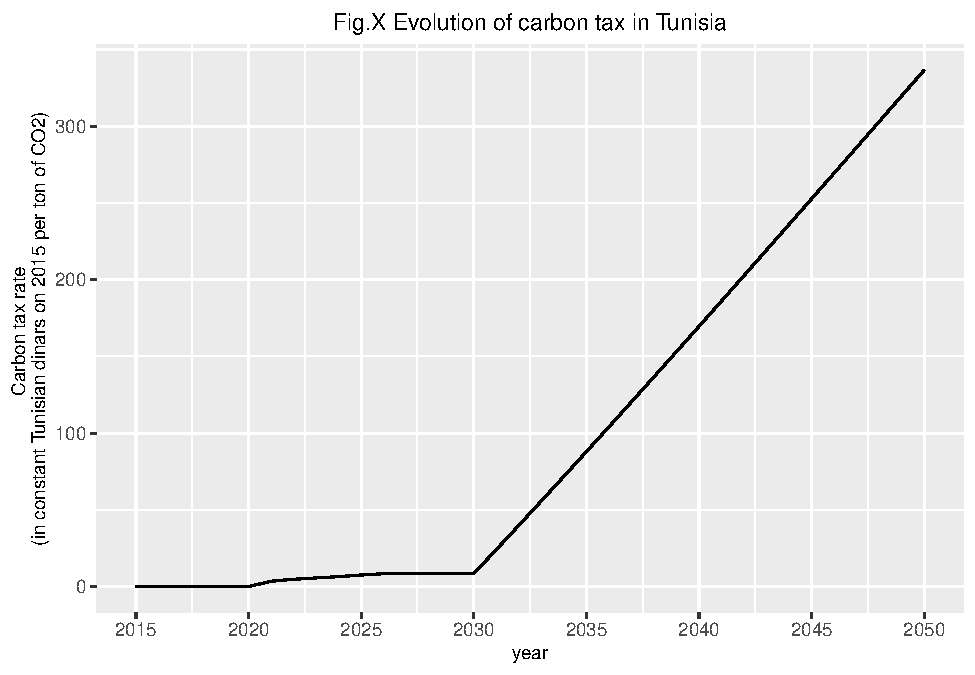
\includegraphics{02-01---Projet-Modélisation-Prospective-ThreeME_files/figure-latex/unnamed-chunk-6-1.pdf}

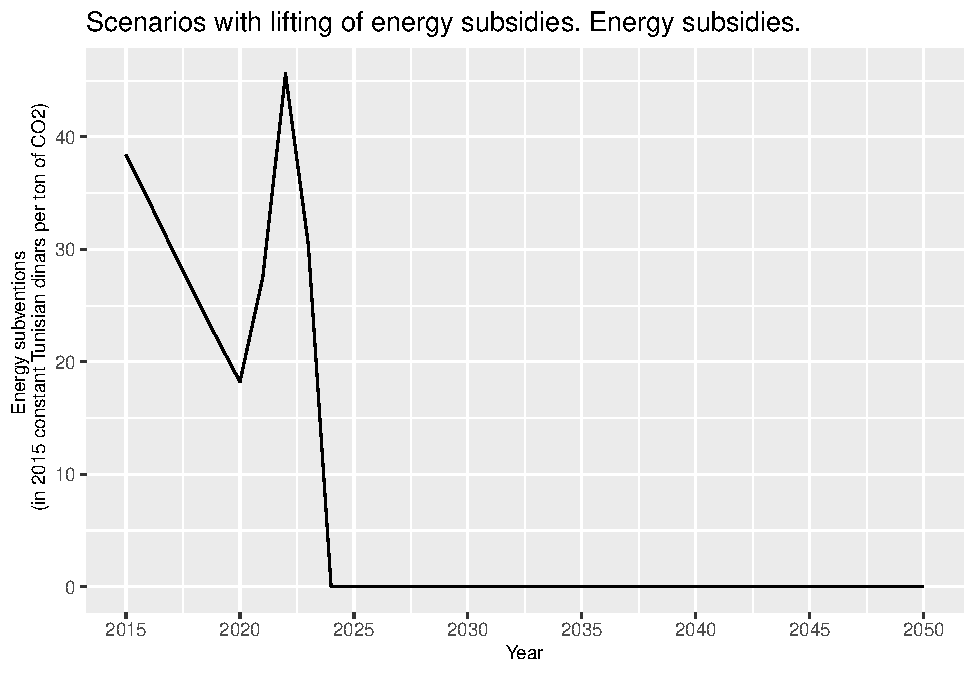
\includegraphics{02-01---Projet-Modélisation-Prospective-ThreeME_files/figure-latex/unnamed-chunk-7-1.pdf}

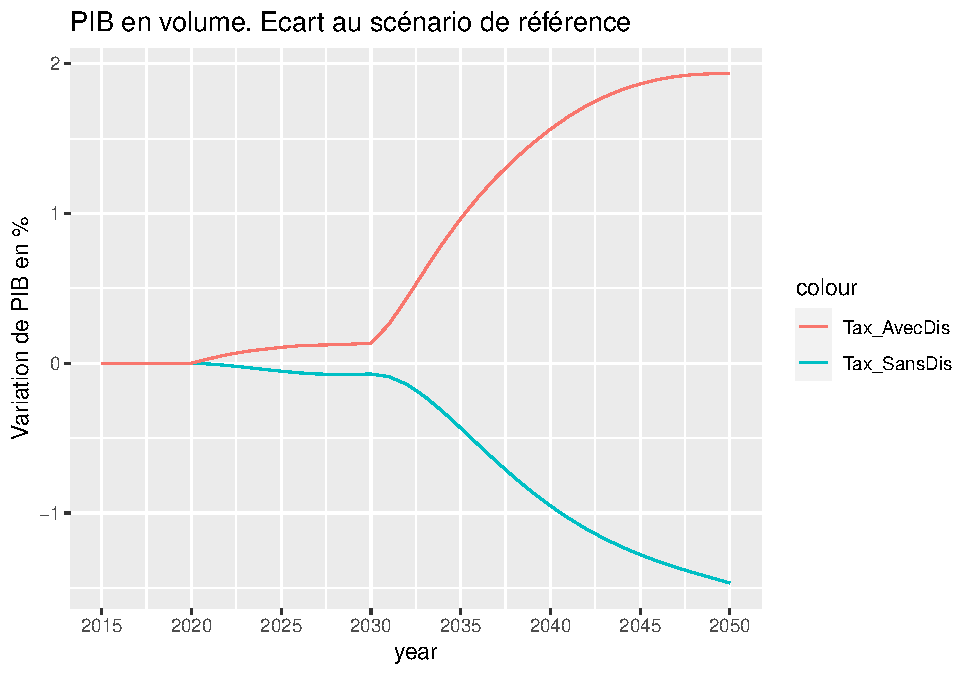
\includegraphics{02-01---Projet-Modélisation-Prospective-ThreeME_files/figure-latex/unnamed-chunk-8-1.pdf}

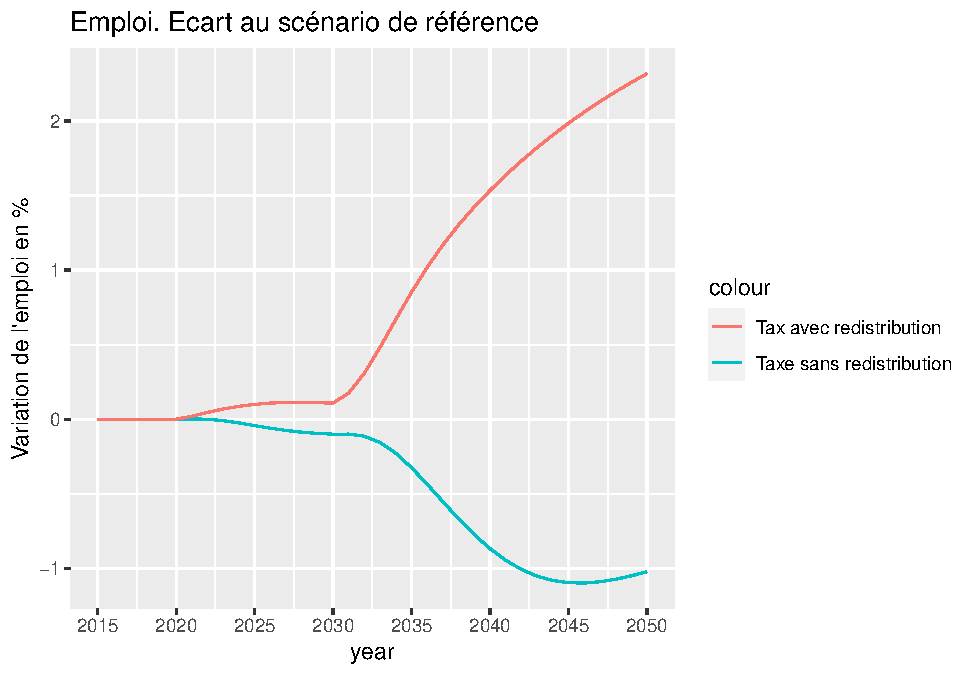
\includegraphics{02-01---Projet-Modélisation-Prospective-ThreeME_files/figure-latex/unnamed-chunk-9-1.pdf}

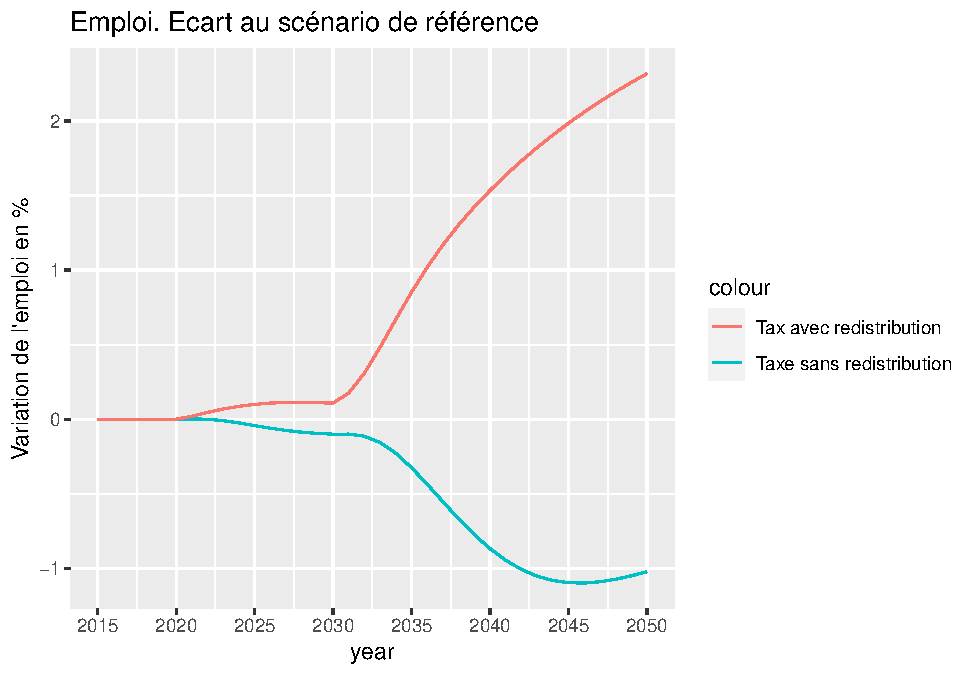
\includegraphics{02-01---Projet-Modélisation-Prospective-ThreeME_files/figure-latex/unnamed-chunk-10-1.pdf}

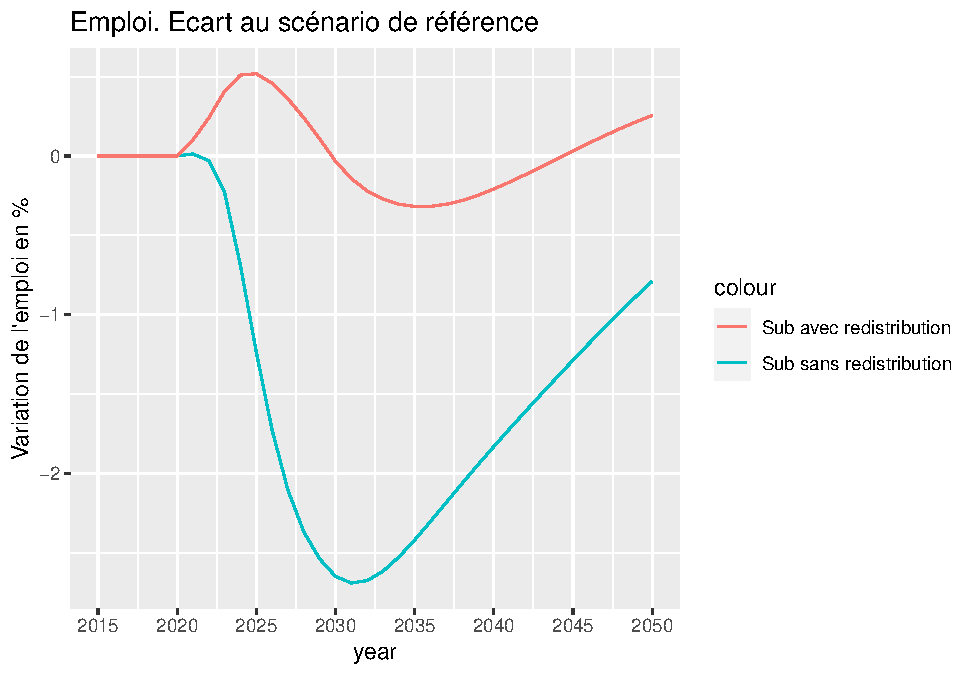
\includegraphics{02-01---Projet-Modélisation-Prospective-ThreeME_files/figure-latex/unnamed-chunk-11-1.pdf}

\hypertarget{b.-production-uxe9nerguxe9tique-par-uxe9nergies}{%
\subsection{B. Production énergétique par
énergies}\label{b.-production-uxe9nerguxe9tique-par-uxe9nergies}}

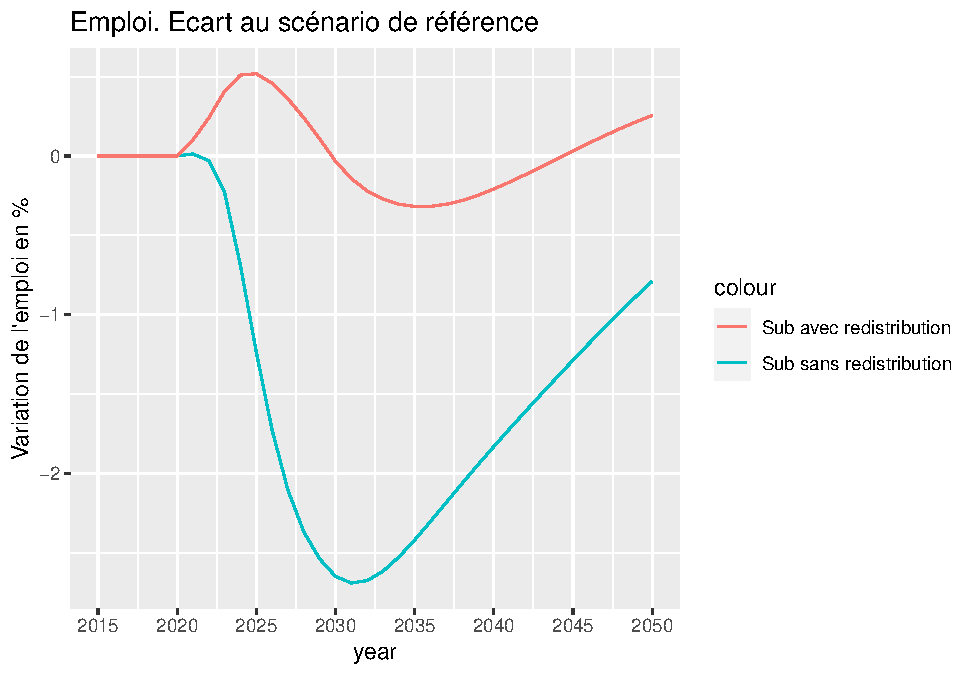
\includegraphics{02-01---Projet-Modélisation-Prospective-ThreeME_files/figure-latex/unnamed-chunk-12-1.pdf}

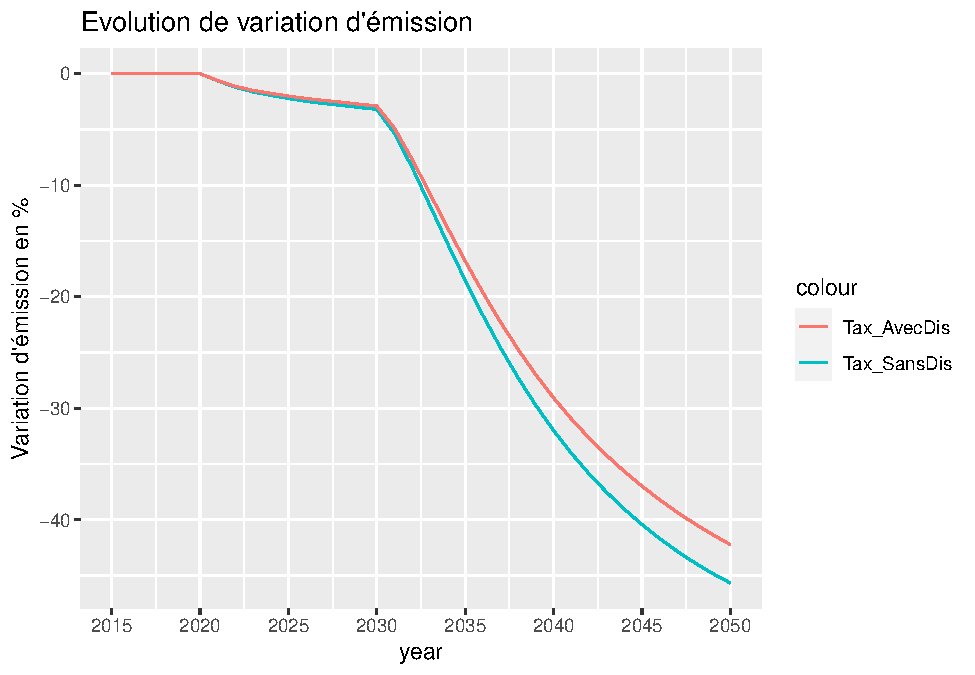
\includegraphics{02-01---Projet-Modélisation-Prospective-ThreeME_files/figure-latex/unnamed-chunk-13-1.pdf}

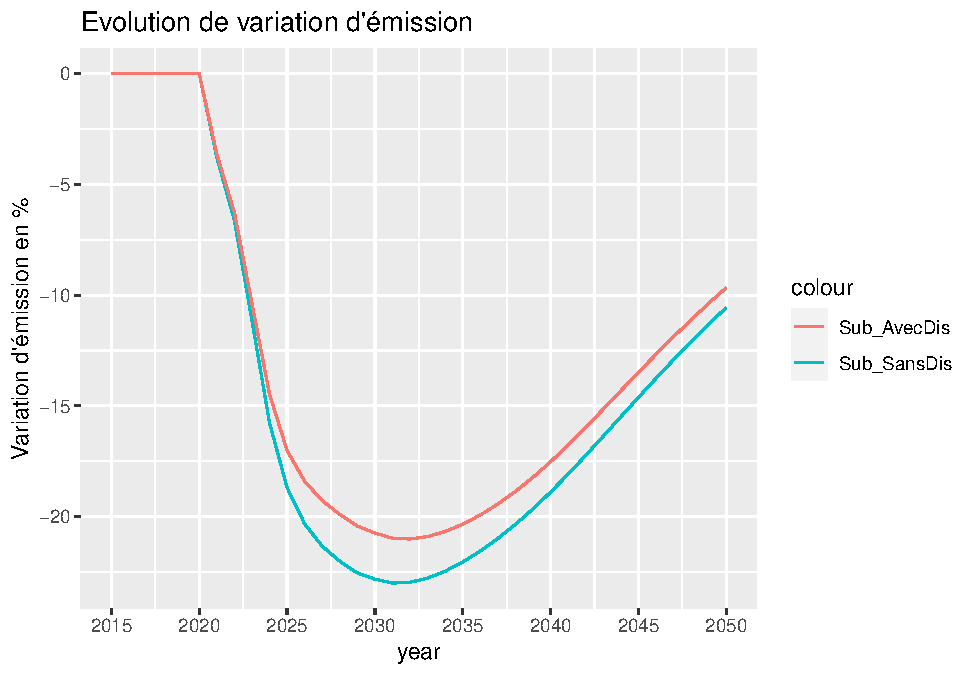
\includegraphics{02-01---Projet-Modélisation-Prospective-ThreeME_files/figure-latex/unnamed-chunk-14-1.pdf}

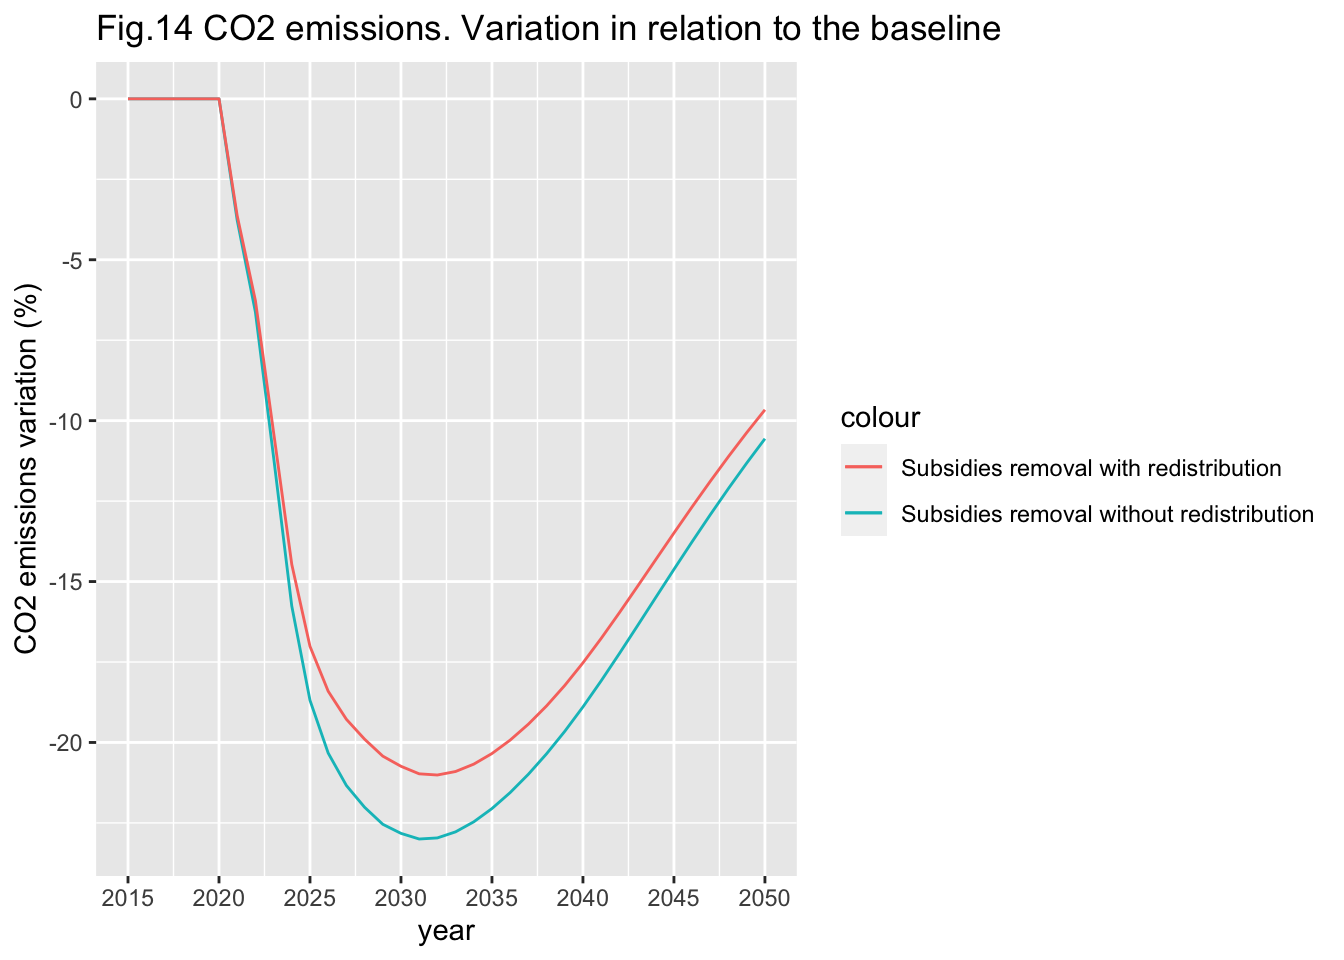
\includegraphics{02-01---Projet-Modélisation-Prospective-ThreeME_files/figure-latex/unnamed-chunk-15-1.pdf}

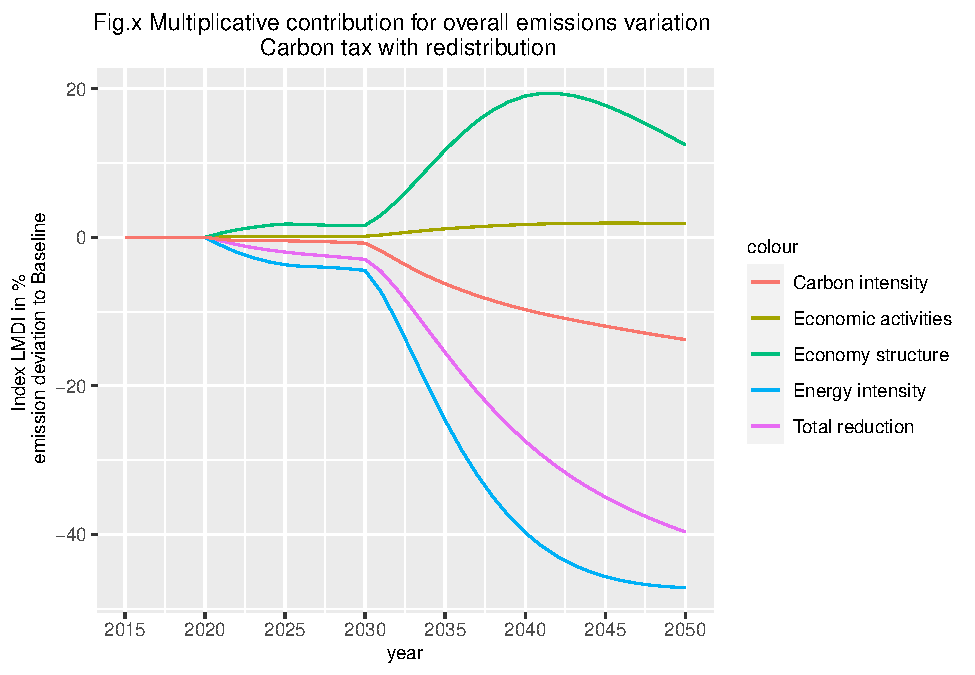
\includegraphics{02-01---Projet-Modélisation-Prospective-ThreeME_files/figure-latex/unnamed-chunk-16-1.pdf}

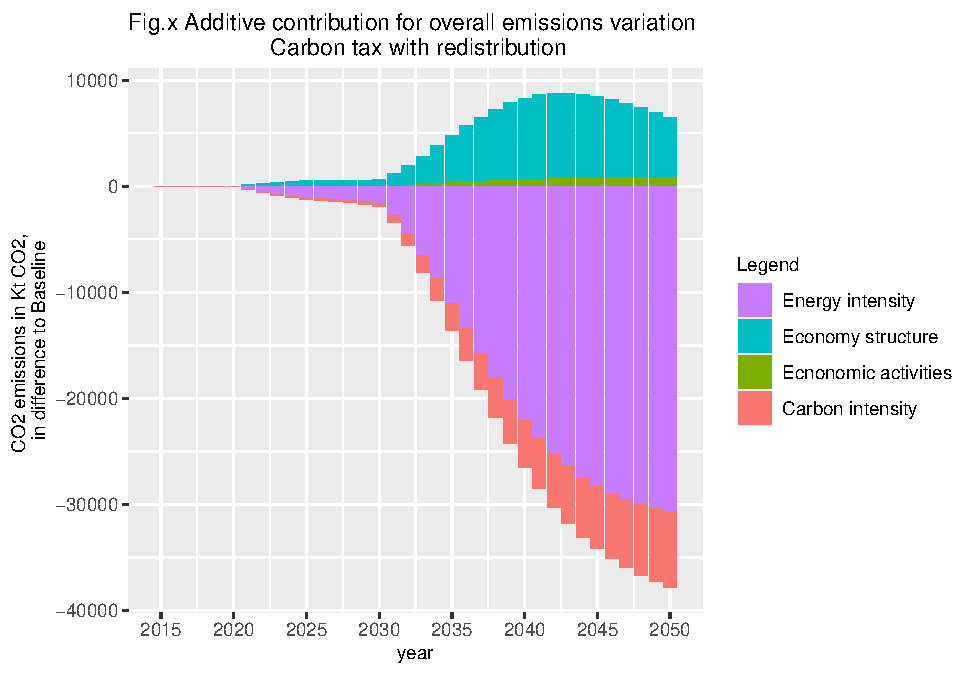
\includegraphics{02-01---Projet-Modélisation-Prospective-ThreeME_files/figure-latex/unnamed-chunk-17-1.pdf}

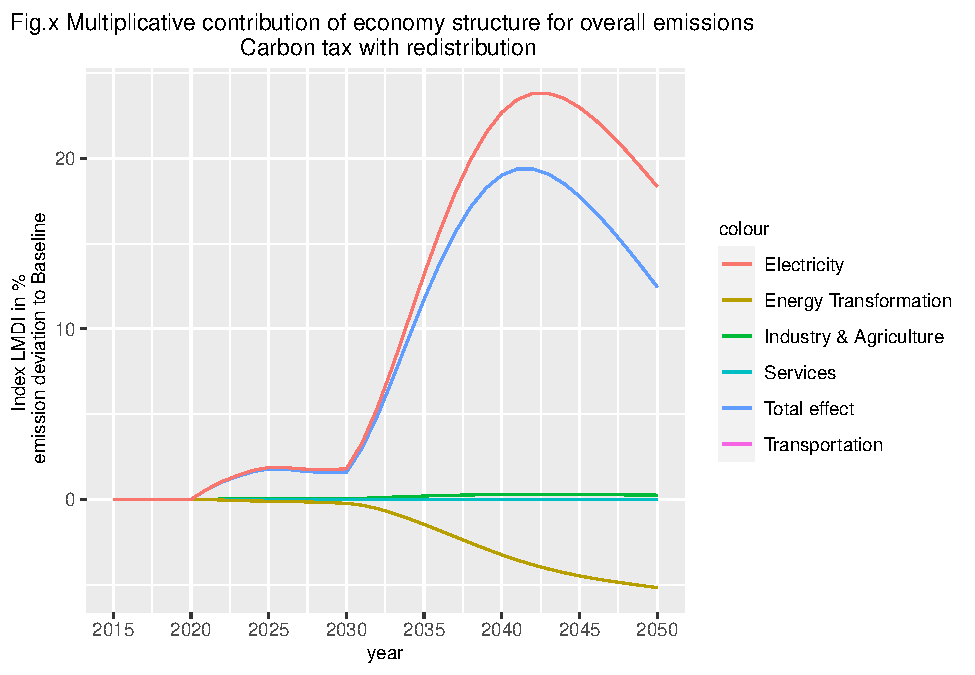
\includegraphics{02-01---Projet-Modélisation-Prospective-ThreeME_files/figure-latex/unnamed-chunk-18-1.pdf}

\hypertarget{c.-consommation-finale-uxe9nerguxe9tique-par-uxe9nergies}{%
\subsection{C. Consommation finale énergétique par
énergies}\label{c.-consommation-finale-uxe9nerguxe9tique-par-uxe9nergies}}

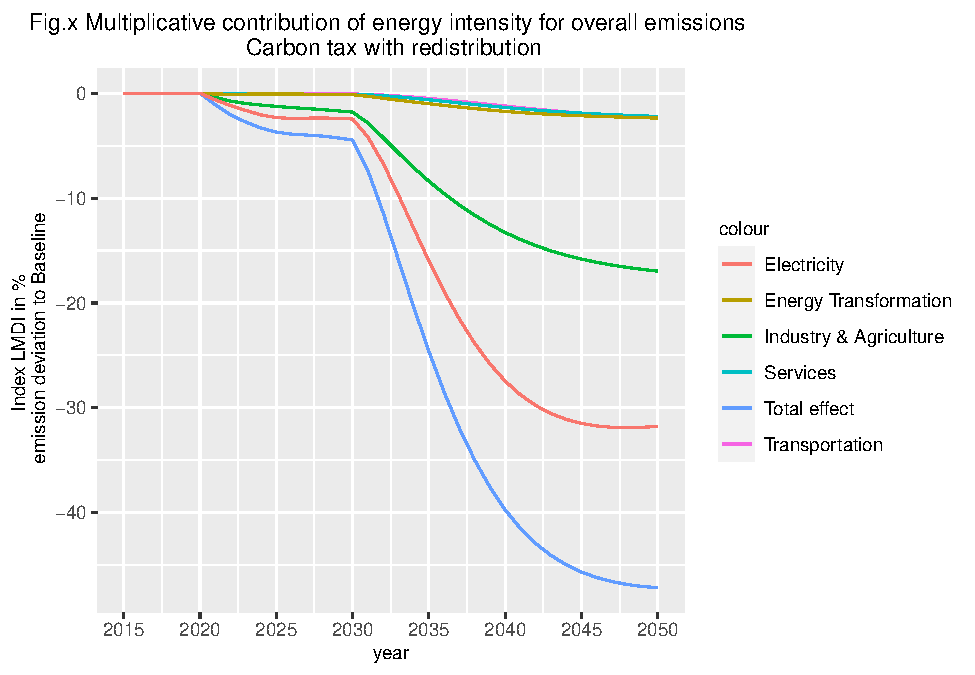
\includegraphics{02-01---Projet-Modélisation-Prospective-ThreeME_files/figure-latex/unnamed-chunk-19-1.pdf}

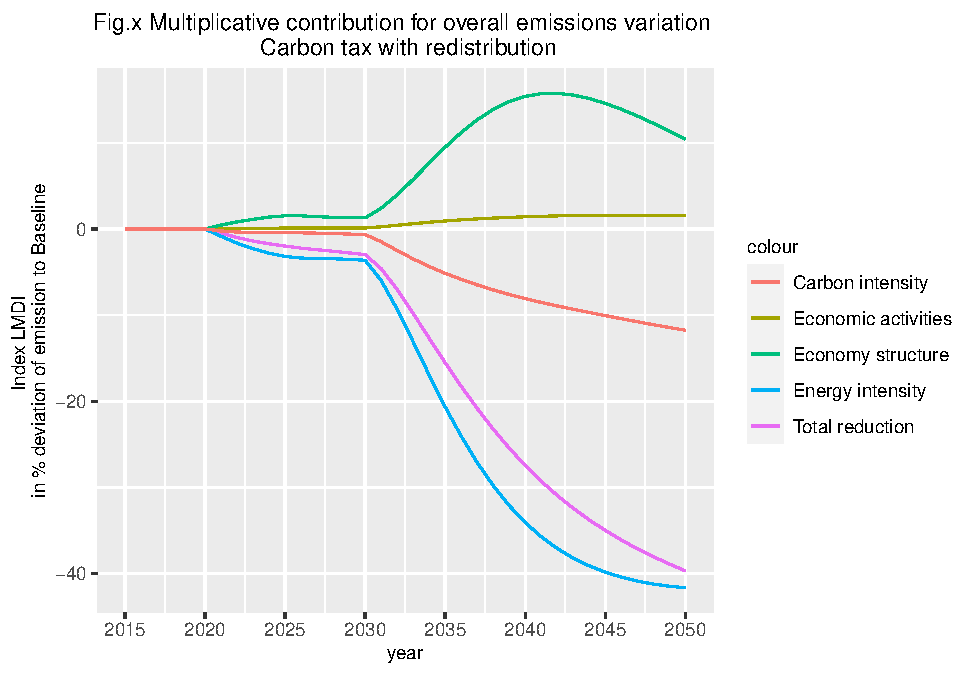
\includegraphics{02-01---Projet-Modélisation-Prospective-ThreeME_files/figure-latex/unnamed-chunk-20-1.pdf}

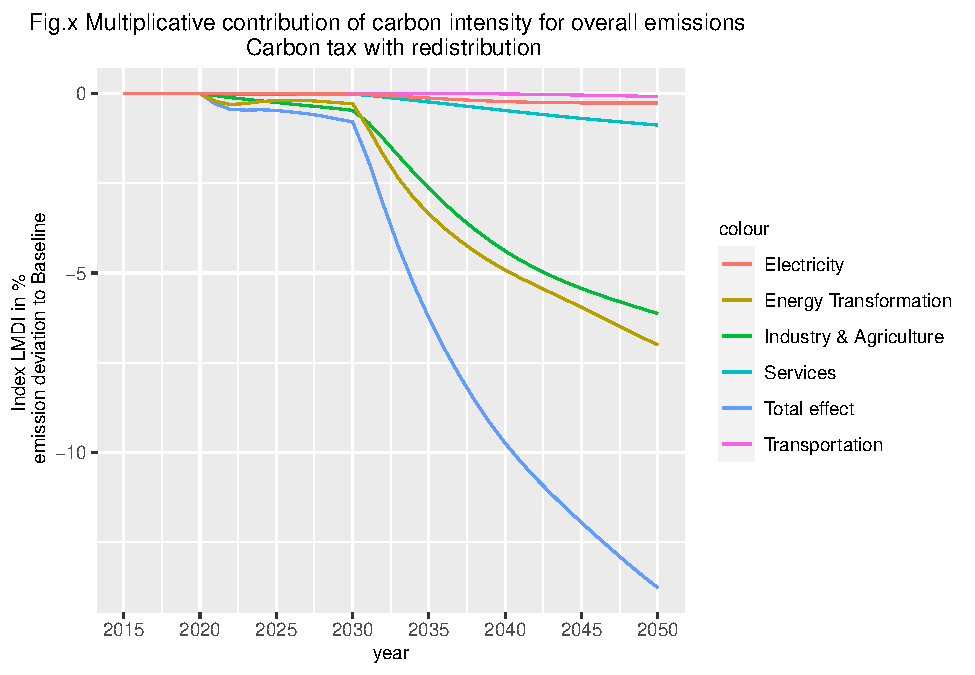
\includegraphics{02-01---Projet-Modélisation-Prospective-ThreeME_files/figure-latex/unnamed-chunk-21-1.pdf}

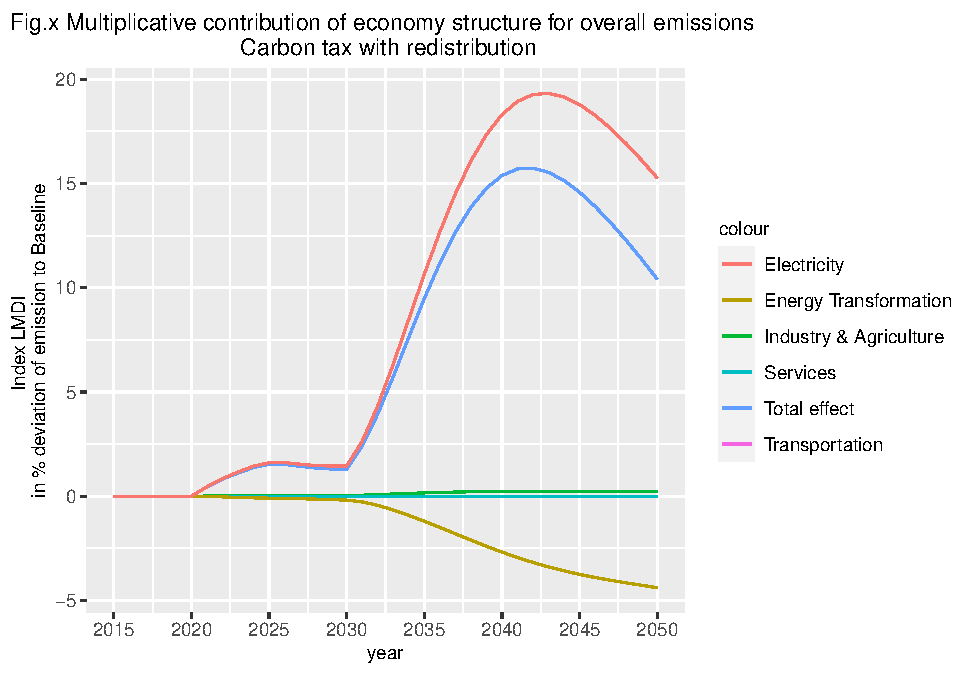
\includegraphics{02-01---Projet-Modélisation-Prospective-ThreeME_files/figure-latex/unnamed-chunk-22-1.pdf}

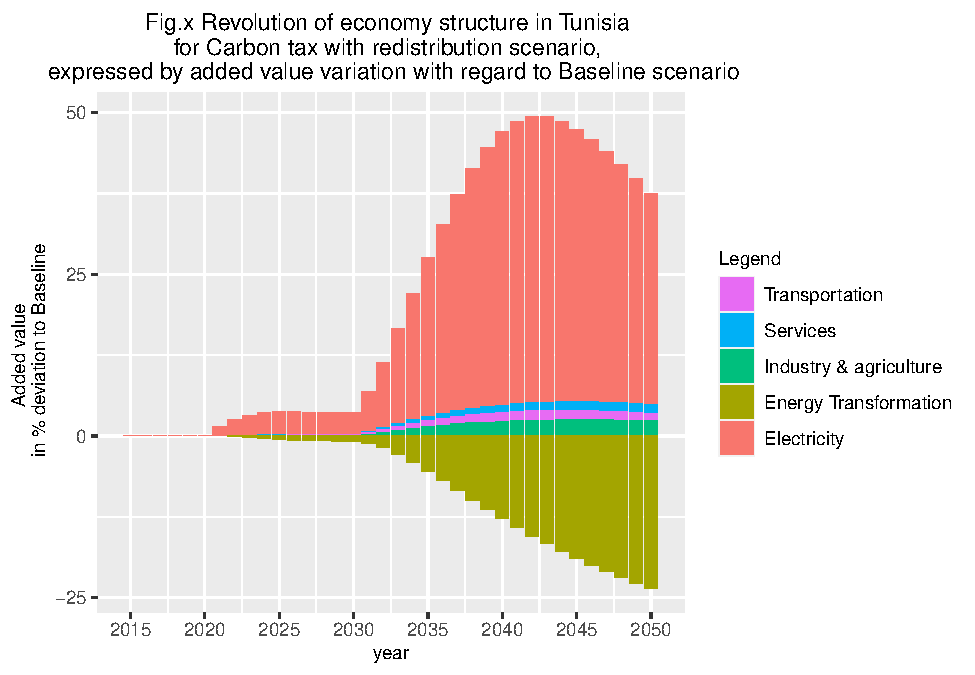
\includegraphics{02-01---Projet-Modélisation-Prospective-ThreeME_files/figure-latex/unnamed-chunk-23-1.pdf}

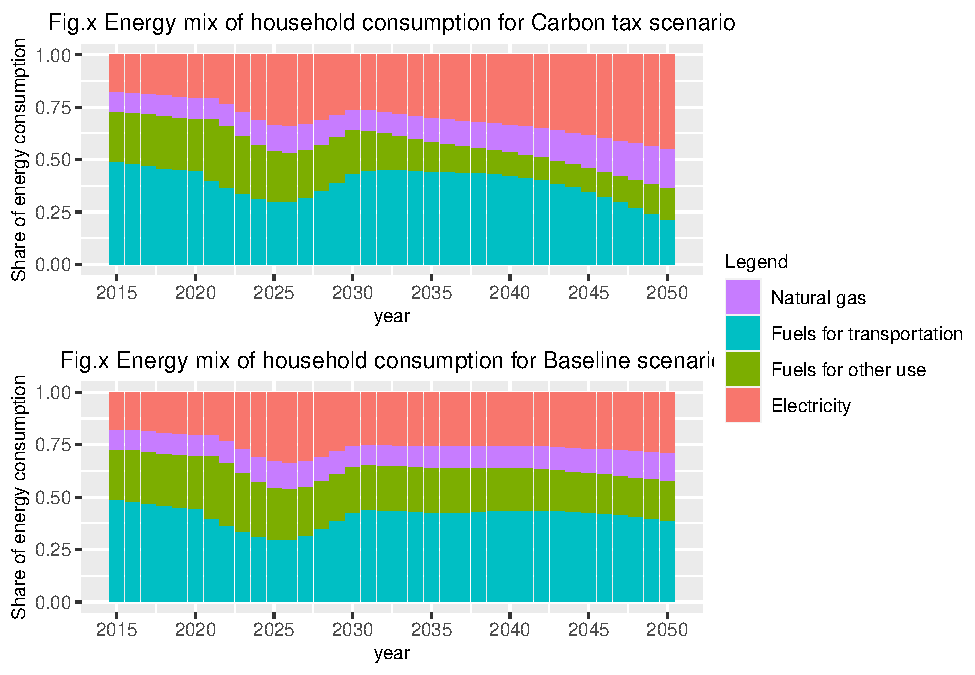
\includegraphics{02-01---Projet-Modélisation-Prospective-ThreeME_files/figure-latex/unnamed-chunk-24-1.pdf}

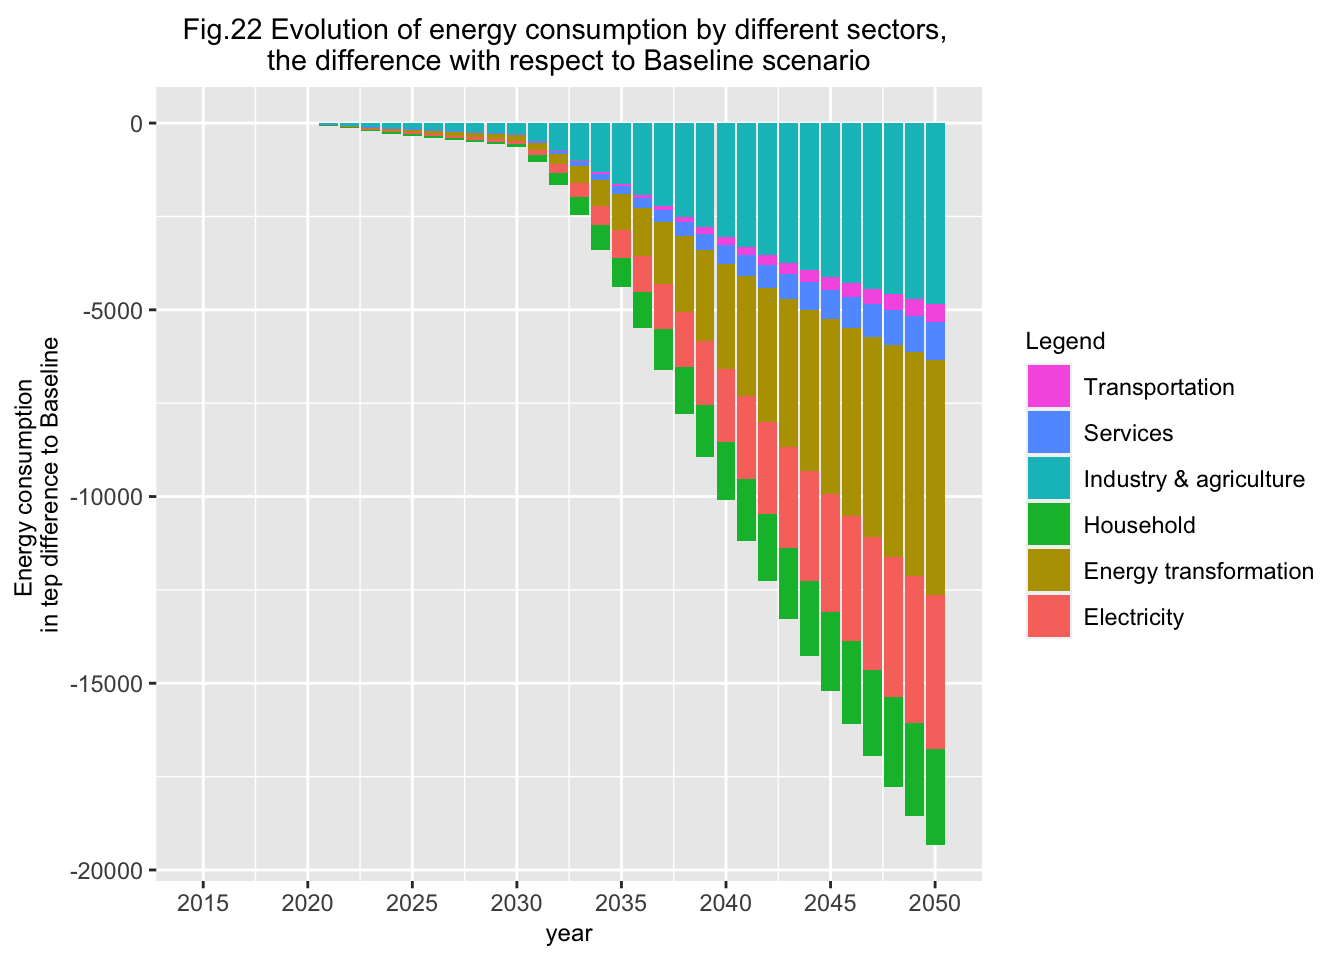
\includegraphics{02-01---Projet-Modélisation-Prospective-ThreeME_files/figure-latex/unnamed-chunk-25-1.pdf}

\hypertarget{iii.-analyse-didentituxe9-kaya}{%
\section{III. Analyse d'identité
Kaya}\label{iii.-analyse-didentituxe9-kaya}}

On a modifié l'identité de Kaya pour qu'elle soit plus cohérente avec
notre étude:

\[ Émission_{CO_2} = VA \times \Sigma(\frac{VA_i}{VA} \times \frac{CE_i}{VA_i} \times \frac{EM_i}{CE_i}) = VA \times\Sigma(S_iI_iU_i)\]

où, VA est la valeur ajoutée totale dans l'économie, \(VA_i\) est la
valeur ajoutée dans secteur \(i\), \(CE_i\) est la consommation
énergétique dans secteur \(i\), \(EM_i\) est l'émission de \(CO_2\) dans
secteur \(i\). On a alors 4 indicateurs qui servent à expliquer la
variation d'émission de \(CO_2\): \(S = \Sigma\frac{VA_i}{VA}\),
\(I = \Sigma\frac{CE_i}{VA_i}\), \(U = \Sigma\frac{EM_i}{CE_i}\) sont,
respectivement, la structure écnomique, l'intensité énergétique et
l'intensité carbone.

\begin{Shaded}
\begin{Highlighting}[]
\CommentTok{\# Decomposition multiplicative}

\NormalTok{name }\OtherTok{\textless{}{-}} \FunctionTok{c}\NormalTok{(}\StringTok{"D1"}\NormalTok{,}\StringTok{"D2"}\NormalTok{,}\StringTok{"D3"}\NormalTok{,}\StringTok{"D4"}\NormalTok{,}\StringTok{"D5"}\NormalTok{,}\StringTok{"D6"}\NormalTok{)}
\NormalTok{secteur }\OtherTok{\textless{}{-}} \FunctionTok{c}\NormalTok{(}\StringTok{"ems\_ci\_co2\_ind\_2"}\NormalTok{,}\StringTok{"ems\_ci\_co2\_trsp\_2"}\NormalTok{,}\StringTok{"ems\_ci\_co2\_ser\_2"}\NormalTok{,}\StringTok{"ems\_ci\_co2\_trsf\_2"}\NormalTok{,}\StringTok{"ems\_ci\_co2\_ele\_2"}\NormalTok{)}
\NormalTok{secteur0 }\OtherTok{\textless{}{-}} \FunctionTok{c}\NormalTok{(}\StringTok{"ems\_ci\_co2\_ind\_0"}\NormalTok{,}\StringTok{"ems\_ci\_co2\_trsp\_0"}\NormalTok{,}\StringTok{"ems\_ci\_co2\_ser\_0"}\NormalTok{,}\StringTok{"ems\_ci\_co2\_trsf\_0"}\NormalTok{,}\StringTok{"ems\_ci\_co2\_ele\_0"}\NormalTok{)}
\NormalTok{kayaname }\OtherTok{\textless{}{-}} \FunctionTok{c}\NormalTok{(}\StringTok{"S\_ind"}\NormalTok{,}\StringTok{"S\_trsp"}\NormalTok{,}\StringTok{"S\_ser"}\NormalTok{,}\StringTok{"S\_trsf"}\NormalTok{,}\StringTok{"S\_ele"}\NormalTok{,}\StringTok{"I\_ind"}\NormalTok{,}\StringTok{"I\_trsp"}\NormalTok{,}\StringTok{"I\_ser"}\NormalTok{,}\StringTok{"I\_trsf"}\NormalTok{,}\StringTok{"I\_ele"}\NormalTok{,}\StringTok{"U\_ind"}\NormalTok{,}\StringTok{"U\_trsp"}\NormalTok{,}\StringTok{"U\_ser"}\NormalTok{,}\StringTok{"U\_trsf"}\NormalTok{,}\StringTok{"U\_ele"}\NormalTok{,}\StringTok{"VA"}\NormalTok{,}\StringTok{"ind"}\NormalTok{,}\StringTok{"trsp"}\NormalTok{,}\StringTok{"ser"}\NormalTok{,}\StringTok{"trsf"}\NormalTok{,}\StringTok{"ele"}\NormalTok{,}\StringTok{"S"}\NormalTok{,}\StringTok{"I"}\NormalTok{,}\StringTok{"U"}\NormalTok{)}

\ControlFlowTok{for}\NormalTok{ (i }\ControlFlowTok{in} \DecValTok{1}\SpecialCharTok{:}\DecValTok{6}\NormalTok{) \{}
  
\NormalTok{  w }\OtherTok{\textless{}{-}} \FunctionTok{as.data.frame}\NormalTok{(}\FunctionTok{array}\NormalTok{(,}\AttributeTok{dim=}\FunctionTok{c}\NormalTok{(}\DecValTok{36}\NormalTok{,}\DecValTok{16}\NormalTok{)))}
  \ControlFlowTok{for}\NormalTok{ (j }\ControlFlowTok{in} \DecValTok{1}\SpecialCharTok{:}\DecValTok{5}\NormalTok{) \{}
\NormalTok{  w[,}\FunctionTok{c}\NormalTok{(j,j}\SpecialCharTok{+}\DecValTok{5}\NormalTok{,j}\SpecialCharTok{+}\DecValTok{10}\NormalTok{)] }\OtherTok{\textless{}{-}}\NormalTok{ ((DataBase[[i]][,secteur[j]]}\SpecialCharTok{{-}}\NormalTok{Baseline[,secteur0[j]])}\SpecialCharTok{/}
          \FunctionTok{log}\NormalTok{(DataBase[[i]][,secteur[j]]}\SpecialCharTok{/}\NormalTok{Baseline[,secteur0[j]]))}\SpecialCharTok{/}
\NormalTok{     ((DataBase[[i]][,}\StringTok{"ems\_ci\_co2\_2"}\NormalTok{] }\SpecialCharTok{{-}}\NormalTok{ Baseline[,}\StringTok{"ems\_ci\_co2\_0"}\NormalTok{])}\SpecialCharTok{/}
       \FunctionTok{log}\NormalTok{(DataBase[[i]][,}\StringTok{"ems\_ci\_co2\_2"}\NormalTok{]}\SpecialCharTok{/}\NormalTok{Baseline[,}\StringTok{"ems\_ci\_co2\_0"}\NormalTok{]))}
\NormalTok{  \}}
\NormalTok{  w[,}\DecValTok{16}\NormalTok{] }\OtherTok{\textless{}{-}}\NormalTok{ w[,}\DecValTok{1}\NormalTok{]}\SpecialCharTok{+}\NormalTok{ w[,}\DecValTok{2}\NormalTok{]}\SpecialCharTok{+}\NormalTok{ w[,}\DecValTok{3}\NormalTok{]}\SpecialCharTok{+}\NormalTok{ w[,}\DecValTok{4}\NormalTok{]}\SpecialCharTok{+}\NormalTok{ w[,}\DecValTok{5}\NormalTok{]}
\NormalTok{  data }\OtherTok{\textless{}{-}} \FunctionTok{exp}\NormalTok{(w}\SpecialCharTok{*}\FunctionTok{log}\NormalTok{(Kaya\_Base[[i]]}\SpecialCharTok{/}\NormalTok{KAYA\_Baseline))}
\NormalTok{  data }\OtherTok{\textless{}{-}} \FunctionTok{rapply}\NormalTok{( data, }\AttributeTok{f=}\ControlFlowTok{function}\NormalTok{(x) }\FunctionTok{ifelse}\NormalTok{(}\FunctionTok{is.nan}\NormalTok{(x),}\DecValTok{1}\NormalTok{,x), }\AttributeTok{how=}\StringTok{"replace"}\NormalTok{ )}
  
  \ControlFlowTok{for}\NormalTok{ (k }\ControlFlowTok{in} \DecValTok{1}\SpecialCharTok{:}\DecValTok{8}\NormalTok{) \{}
    \ControlFlowTok{if}\NormalTok{ (k }\SpecialCharTok{\textless{}} \DecValTok{6}\NormalTok{) \{}
\NormalTok{      data }\OtherTok{\textless{}{-}}\NormalTok{ data }\SpecialCharTok{\%\textgreater{}\%} \FunctionTok{add\_column}\NormalTok{(}\AttributeTok{newColname =}\NormalTok{ data[,k] }\SpecialCharTok{*}\NormalTok{ data[,k}\SpecialCharTok{+}\DecValTok{5}\NormalTok{] }\SpecialCharTok{*}\NormalTok{ data[,k}\SpecialCharTok{+}\DecValTok{10}\NormalTok{]) }
\NormalTok{    \}}
    \ControlFlowTok{else} \ControlFlowTok{if}\NormalTok{ (k }\SpecialCharTok{==} \DecValTok{6}\NormalTok{) \{}
\NormalTok{      data }\OtherTok{\textless{}{-}}\NormalTok{ data }\SpecialCharTok{\%\textgreater{}\%} \FunctionTok{add\_column}\NormalTok{(}\AttributeTok{newColname =}\NormalTok{ data[,k}\DecValTok{{-}5}\NormalTok{]}\SpecialCharTok{*}\NormalTok{data[,k}\DecValTok{{-}4}\NormalTok{]}\SpecialCharTok{*}\NormalTok{data[,k}\DecValTok{{-}3}\NormalTok{]}\SpecialCharTok{*}\NormalTok{data[,k}\DecValTok{{-}2}\NormalTok{]}\SpecialCharTok{*}\NormalTok{data[,k}\DecValTok{{-}1}\NormalTok{]) }
\NormalTok{    \}}
    \ControlFlowTok{else} \ControlFlowTok{if}\NormalTok{ (k }\SpecialCharTok{==} \DecValTok{7}\NormalTok{) \{}
\NormalTok{      data }\OtherTok{\textless{}{-}}\NormalTok{ data }\SpecialCharTok{\%\textgreater{}\%} \FunctionTok{add\_column}\NormalTok{(}\AttributeTok{newColname =}\NormalTok{ data[,k}\DecValTok{{-}1}\NormalTok{]}\SpecialCharTok{*}\NormalTok{data[,k]}\SpecialCharTok{*}\NormalTok{data[,k}\SpecialCharTok{+}\DecValTok{1}\NormalTok{]}\SpecialCharTok{*}\NormalTok{data[,k}\SpecialCharTok{+}\DecValTok{2}\NormalTok{]}\SpecialCharTok{*}\NormalTok{data[,k}\SpecialCharTok{+}\DecValTok{3}\NormalTok{]) }
\NormalTok{    \}}
    \ControlFlowTok{else} \ControlFlowTok{if}\NormalTok{ (k }\SpecialCharTok{==} \DecValTok{8}\NormalTok{) \{}
\NormalTok{      data }\OtherTok{\textless{}{-}}\NormalTok{ data }\SpecialCharTok{\%\textgreater{}\%} \FunctionTok{add\_column}\NormalTok{(}\AttributeTok{newColname =}\NormalTok{ data[,k}\SpecialCharTok{+}\DecValTok{3}\NormalTok{]}\SpecialCharTok{*}\NormalTok{data[,k}\SpecialCharTok{+}\DecValTok{4}\NormalTok{]}\SpecialCharTok{*}\NormalTok{data[,k}\SpecialCharTok{+}\DecValTok{5}\NormalTok{]}\SpecialCharTok{*}\NormalTok{data[,k}\SpecialCharTok{+}\DecValTok{6}\NormalTok{]}\SpecialCharTok{*}\NormalTok{data[,k}\SpecialCharTok{+}\DecValTok{7}\NormalTok{]) }
\NormalTok{    \}}
\NormalTok{  \}}
  
  \FunctionTok{colnames}\NormalTok{(data) }\OtherTok{\textless{}{-}}\NormalTok{ kayaname}
\NormalTok{  data}\SpecialCharTok{$}\NormalTok{year }\OtherTok{\textless{}{-}} \FunctionTok{c}\NormalTok{(}\DecValTok{2015}\SpecialCharTok{:}\DecValTok{2050}\NormalTok{)}
\NormalTok{  data }\OtherTok{\textless{}{-}}\NormalTok{ (data }\SpecialCharTok{{-}} \DecValTok{1}\NormalTok{) }\SpecialCharTok{*} \DecValTok{100}
\NormalTok{  jin }\OtherTok{\textless{}{-}}\NormalTok{ name[i]}
  \FunctionTok{assign}\NormalTok{(jin,data)}
\NormalTok{\}}

\NormalTok{Det }\OtherTok{\textless{}{-}} \FunctionTok{list}\NormalTok{(D1,D2,D3,D4,D5,D6)}

\FunctionTok{rm}\NormalTok{(i,j,jin,name,kayaname,secteur,secteur0,w,data,D1,D2,D3,D4,D5,D6)}
\end{Highlighting}
\end{Shaded}

\begin{Shaded}
\begin{Highlighting}[]
\CommentTok{\# Decomposition additive}
\NormalTok{name }\OtherTok{\textless{}{-}} \FunctionTok{c}\NormalTok{(}\StringTok{"D1"}\NormalTok{,}\StringTok{"D2"}\NormalTok{,}\StringTok{"D3"}\NormalTok{,}\StringTok{"D4"}\NormalTok{,}\StringTok{"D5"}\NormalTok{,}\StringTok{"D6"}\NormalTok{)}
\NormalTok{secteur }\OtherTok{\textless{}{-}} \FunctionTok{c}\NormalTok{(}\StringTok{"ems\_ci\_co2\_ind\_2"}\NormalTok{,}\StringTok{"ems\_ci\_co2\_trsp\_2"}\NormalTok{,}\StringTok{"ems\_ci\_co2\_ser\_2"}\NormalTok{,}\StringTok{"ems\_ci\_co2\_trsf\_2"}\NormalTok{,}\StringTok{"ems\_ci\_co2\_ele\_2"}\NormalTok{)}
\NormalTok{secteur0 }\OtherTok{\textless{}{-}} \FunctionTok{c}\NormalTok{(}\StringTok{"ems\_ci\_co2\_ind\_0"}\NormalTok{,}\StringTok{"ems\_ci\_co2\_trsp\_0"}\NormalTok{,}\StringTok{"ems\_ci\_co2\_ser\_0"}\NormalTok{,}\StringTok{"ems\_ci\_co2\_trsf\_0"}\NormalTok{,}\StringTok{"ems\_ci\_co2\_ele\_0"}\NormalTok{)}
\NormalTok{kayaname }\OtherTok{\textless{}{-}} \FunctionTok{c}\NormalTok{(}\StringTok{"S\_ind"}\NormalTok{,}\StringTok{"S\_trsp"}\NormalTok{,}\StringTok{"S\_ser"}\NormalTok{,}\StringTok{"S\_trsf"}\NormalTok{,}\StringTok{"S\_ele"}\NormalTok{,}\StringTok{"I\_ind"}\NormalTok{,}\StringTok{"I\_trsp"}\NormalTok{,}\StringTok{"I\_ser"}\NormalTok{,}\StringTok{"I\_trsf"}\NormalTok{,}\StringTok{"I\_ele"}\NormalTok{,}\StringTok{"U\_ind"}\NormalTok{,}\StringTok{"U\_trsp"}\NormalTok{,}\StringTok{"U\_ser"}\NormalTok{,}\StringTok{"U\_trsf"}\NormalTok{,}\StringTok{"U\_ele"}\NormalTok{,}\StringTok{"VA"}\NormalTok{,}\StringTok{"ind"}\NormalTok{,}\StringTok{"trsp"}\NormalTok{,}\StringTok{"ser"}\NormalTok{,}\StringTok{"trsf"}\NormalTok{,}\StringTok{"ele"}\NormalTok{,}\StringTok{"S"}\NormalTok{,}\StringTok{"I"}\NormalTok{,}\StringTok{"U"}\NormalTok{)}

\ControlFlowTok{for}\NormalTok{ (i }\ControlFlowTok{in} \DecValTok{1}\SpecialCharTok{:}\DecValTok{6}\NormalTok{) \{}
  
\NormalTok{  w }\OtherTok{\textless{}{-}} \FunctionTok{as.data.frame}\NormalTok{(}\FunctionTok{array}\NormalTok{(,}\AttributeTok{dim=}\FunctionTok{c}\NormalTok{(}\DecValTok{36}\NormalTok{,}\DecValTok{16}\NormalTok{)))}
  
  \ControlFlowTok{for}\NormalTok{ (j }\ControlFlowTok{in} \DecValTok{1}\SpecialCharTok{:}\DecValTok{5}\NormalTok{) \{}
\NormalTok{    w[,}\FunctionTok{c}\NormalTok{(j,j}\SpecialCharTok{+}\DecValTok{5}\NormalTok{,j}\SpecialCharTok{+}\DecValTok{10}\NormalTok{)] }\OtherTok{\textless{}{-}}\NormalTok{ (DataBase[[i]][,secteur[j]]}\SpecialCharTok{{-}}\NormalTok{Baseline[,secteur0[j]])}\SpecialCharTok{/}
          \FunctionTok{log}\NormalTok{(DataBase[[i]][,secteur[j]]}\SpecialCharTok{/}\NormalTok{Baseline[,secteur0[j]])}
\NormalTok{  \}}
  
\NormalTok{  w[,}\DecValTok{16}\NormalTok{] }\OtherTok{\textless{}{-}}\NormalTok{ w[,}\DecValTok{1}\NormalTok{]}\SpecialCharTok{+}\NormalTok{ w[,}\DecValTok{2}\NormalTok{]}\SpecialCharTok{+}\NormalTok{ w[,}\DecValTok{3}\NormalTok{]}\SpecialCharTok{+}\NormalTok{ w[,}\DecValTok{4}\NormalTok{]}\SpecialCharTok{+}\NormalTok{ w[,}\DecValTok{5}\NormalTok{]}
\NormalTok{  data }\OtherTok{\textless{}{-}}\NormalTok{ w}\SpecialCharTok{*}\FunctionTok{log}\NormalTok{(Kaya\_Base[[i]]}\SpecialCharTok{/}\NormalTok{KAYA\_Baseline)}
\NormalTok{  data }\OtherTok{\textless{}{-}} \FunctionTok{rapply}\NormalTok{( data, }\AttributeTok{f=}\ControlFlowTok{function}\NormalTok{(x) }\FunctionTok{ifelse}\NormalTok{(}\FunctionTok{is.nan}\NormalTok{(x),}\DecValTok{0}\NormalTok{,x), }\AttributeTok{how=}\StringTok{"replace"}\NormalTok{ )}
  
  \ControlFlowTok{for}\NormalTok{ (k }\ControlFlowTok{in} \DecValTok{1}\SpecialCharTok{:}\DecValTok{8}\NormalTok{) \{}
    \ControlFlowTok{if}\NormalTok{ (k }\SpecialCharTok{\textless{}} \DecValTok{6}\NormalTok{) \{}
\NormalTok{      data }\OtherTok{\textless{}{-}}\NormalTok{ data }\SpecialCharTok{\%\textgreater{}\%} \FunctionTok{add\_column}\NormalTok{(}\AttributeTok{newColname =}\NormalTok{ data[,k] }\SpecialCharTok{+}\NormalTok{ data[,k}\SpecialCharTok{+}\DecValTok{5}\NormalTok{] }\SpecialCharTok{+}\NormalTok{ data[,k}\SpecialCharTok{+}\DecValTok{10}\NormalTok{]) }
\NormalTok{    \}}
    \ControlFlowTok{else} \ControlFlowTok{if}\NormalTok{ (k }\SpecialCharTok{==} \DecValTok{6}\NormalTok{) \{}
\NormalTok{      data }\OtherTok{\textless{}{-}}\NormalTok{ data }\SpecialCharTok{\%\textgreater{}\%} \FunctionTok{add\_column}\NormalTok{(}\AttributeTok{newColname =}\NormalTok{ data[,k}\DecValTok{{-}5}\NormalTok{]}\SpecialCharTok{+}\NormalTok{data[,k}\DecValTok{{-}4}\NormalTok{]}\SpecialCharTok{+}\NormalTok{data[,k}\DecValTok{{-}3}\NormalTok{]}\SpecialCharTok{+}\NormalTok{data[,k}\DecValTok{{-}2}\NormalTok{]}\SpecialCharTok{+}\NormalTok{data[,k}\DecValTok{{-}1}\NormalTok{]) }
\NormalTok{    \}}
    \ControlFlowTok{else} \ControlFlowTok{if}\NormalTok{ (k }\SpecialCharTok{==} \DecValTok{7}\NormalTok{) \{}
\NormalTok{      data }\OtherTok{\textless{}{-}}\NormalTok{ data }\SpecialCharTok{\%\textgreater{}\%} \FunctionTok{add\_column}\NormalTok{(}\AttributeTok{newColname =}\NormalTok{ data[,k}\DecValTok{{-}1}\NormalTok{]}\SpecialCharTok{+}\NormalTok{data[,k]}\SpecialCharTok{+}\NormalTok{data[,k}\SpecialCharTok{+}\DecValTok{1}\NormalTok{]}\SpecialCharTok{+}\NormalTok{data[,k}\SpecialCharTok{+}\DecValTok{2}\NormalTok{]}\SpecialCharTok{+}\NormalTok{data[,k}\SpecialCharTok{+}\DecValTok{3}\NormalTok{]) }
\NormalTok{    \}}
    \ControlFlowTok{else} \ControlFlowTok{if}\NormalTok{ (k }\SpecialCharTok{==} \DecValTok{8}\NormalTok{) \{}
\NormalTok{      data }\OtherTok{\textless{}{-}}\NormalTok{ data }\SpecialCharTok{\%\textgreater{}\%} \FunctionTok{add\_column}\NormalTok{(}\AttributeTok{newColname =}\NormalTok{ data[,k}\SpecialCharTok{+}\DecValTok{3}\NormalTok{]}\SpecialCharTok{+}\NormalTok{data[,k}\SpecialCharTok{+}\DecValTok{4}\NormalTok{]}\SpecialCharTok{+}\NormalTok{data[,k}\SpecialCharTok{+}\DecValTok{5}\NormalTok{]}\SpecialCharTok{+}\NormalTok{data[,k}\SpecialCharTok{+}\DecValTok{6}\NormalTok{]}\SpecialCharTok{+}\NormalTok{data[,k}\SpecialCharTok{+}\DecValTok{7}\NormalTok{]) }
\NormalTok{    \}}
\NormalTok{  \}}
  
  \FunctionTok{colnames}\NormalTok{(data) }\OtherTok{\textless{}{-}}\NormalTok{ kayaname}
\NormalTok{  data}\SpecialCharTok{$}\NormalTok{year }\OtherTok{\textless{}{-}} \FunctionTok{c}\NormalTok{(}\DecValTok{2015}\SpecialCharTok{:}\DecValTok{2050}\NormalTok{)}
\NormalTok{  jin }\OtherTok{\textless{}{-}}\NormalTok{ name[i]}
  \FunctionTok{assign}\NormalTok{(jin,data)}
\NormalTok{\}}

\NormalTok{Dif }\OtherTok{\textless{}{-}} \FunctionTok{list}\NormalTok{(D1,D2,D3,D4,D5,D6)}

\FunctionTok{rm}\NormalTok{(i,j,jin,name,secteur,secteur0,w,data,D1,D2,D3,D4,D5,D6)}
\end{Highlighting}
\end{Shaded}

\begin{Shaded}
\begin{Highlighting}[]
\FunctionTok{ggplot}\NormalTok{() }\SpecialCharTok{+} 
  \FunctionTok{geom\_line}\NormalTok{( }\FunctionTok{aes}\NormalTok{(}\AttributeTok{x =}\NormalTok{ Det[[}\DecValTok{1}\NormalTok{]][,}\StringTok{"year"}\NormalTok{],}\AttributeTok{y =}\NormalTok{ S1[,}\StringTok{"ems\_ci\_co2\_2"}\NormalTok{]}\SpecialCharTok{/}\NormalTok{Baseline[,}\StringTok{"ems\_ci\_co2\_0"}\NormalTok{]}\SpecialCharTok{*}\DecValTok{100} \SpecialCharTok{{-}} \DecValTok{100}\NormalTok{, }\AttributeTok{group =} \DecValTok{1}\NormalTok{, }\AttributeTok{color =} \StringTok{"Baisse totale"}\NormalTok{)) }\SpecialCharTok{+} 
  \FunctionTok{geom\_line}\NormalTok{( }\FunctionTok{aes}\NormalTok{(}\AttributeTok{x =}\NormalTok{ Det[[}\DecValTok{1}\NormalTok{]][,}\StringTok{"year"}\NormalTok{],}\AttributeTok{y =}\NormalTok{ Det[[}\DecValTok{6}\NormalTok{]][,}\StringTok{"VA"}\NormalTok{], }\AttributeTok{group =} \DecValTok{1}\NormalTok{, }\AttributeTok{color =} \StringTok{"Activité économique"}\NormalTok{)) }\SpecialCharTok{+} 
  \FunctionTok{geom\_line}\NormalTok{( }\FunctionTok{aes}\NormalTok{(}\AttributeTok{x =}\NormalTok{ Det[[}\DecValTok{1}\NormalTok{]][,}\StringTok{"year"}\NormalTok{],}\AttributeTok{y =}\NormalTok{ Det[[}\DecValTok{6}\NormalTok{]][,}\StringTok{"U"}\NormalTok{], }\AttributeTok{group =} \DecValTok{1}\NormalTok{, }\AttributeTok{color =} \StringTok{"Intensité carbone"}\NormalTok{)) }\SpecialCharTok{+} 
  \FunctionTok{geom\_line}\NormalTok{( }\FunctionTok{aes}\NormalTok{(}\AttributeTok{x =}\NormalTok{ Det[[}\DecValTok{1}\NormalTok{]][,}\StringTok{"year"}\NormalTok{],}\AttributeTok{y =}\NormalTok{ Det[[}\DecValTok{6}\NormalTok{]][,}\StringTok{"S"}\NormalTok{], }\AttributeTok{group =} \DecValTok{1}\NormalTok{, }\AttributeTok{color =} \StringTok{"Structure économique"}\NormalTok{)) }\SpecialCharTok{+} 
  \FunctionTok{geom\_line}\NormalTok{( }\FunctionTok{aes}\NormalTok{(}\AttributeTok{x =}\NormalTok{ Det[[}\DecValTok{1}\NormalTok{]][,}\StringTok{"year"}\NormalTok{],}\AttributeTok{y =}\NormalTok{ Det[[}\DecValTok{6}\NormalTok{]][,}\StringTok{"I"}\NormalTok{], }\AttributeTok{group =} \DecValTok{1}\NormalTok{, }\AttributeTok{color =} \StringTok{"Intensité énergétique"}\NormalTok{)) }\SpecialCharTok{+} 
  \FunctionTok{labs}\NormalTok{(}\AttributeTok{x =} \StringTok{"year"}\NormalTok{, }\AttributeTok{y =} \StringTok{"Variation d\textquotesingle{}émission CO2"}\NormalTok{, }\AttributeTok{title =} \StringTok{"Contribution multiplicative sur l\textquotesingle{}émission {-} Melange politique"}\NormalTok{) }\SpecialCharTok{+}
  \FunctionTok{scale\_x\_continuous}\NormalTok{(}\AttributeTok{breaks=}\FunctionTok{seq}\NormalTok{(}\DecValTok{2015}\NormalTok{,}\DecValTok{2050}\NormalTok{,}\DecValTok{5}\NormalTok{))}
\end{Highlighting}
\end{Shaded}

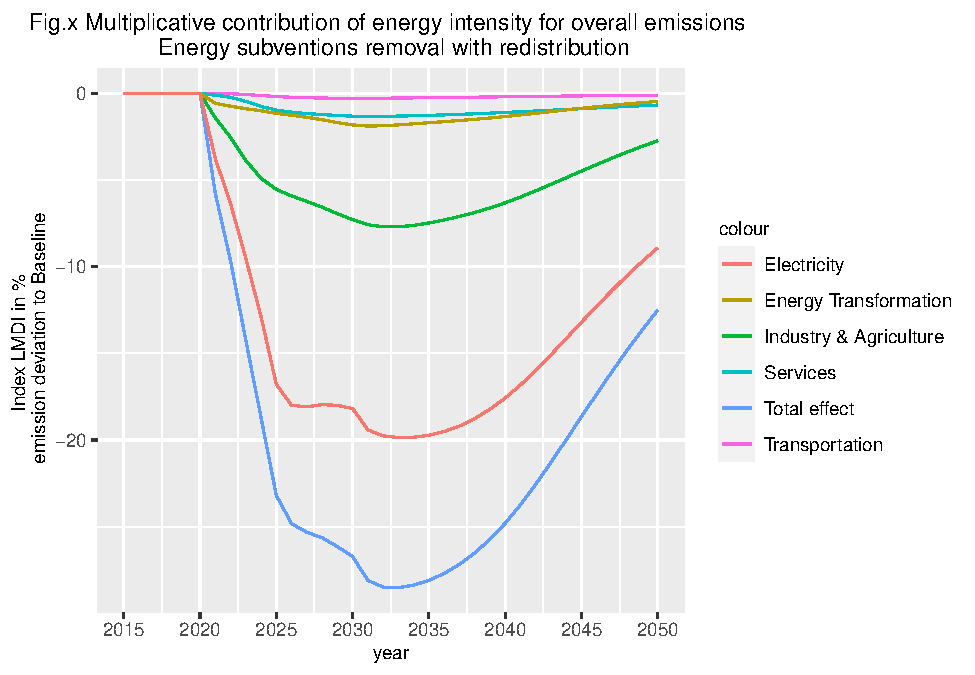
\includegraphics{02-01---Projet-Modélisation-Prospective-ThreeME_files/figure-latex/unnamed-chunk-29-1.pdf}

\begin{Shaded}
\begin{Highlighting}[]
\FunctionTok{ggplot}\NormalTok{() }\SpecialCharTok{+} 
  \FunctionTok{geom\_line}\NormalTok{( }\FunctionTok{aes}\NormalTok{(}\AttributeTok{x =}\NormalTok{ Det[[}\DecValTok{5}\NormalTok{]][,}\StringTok{"year"}\NormalTok{],}\AttributeTok{y =}\NormalTok{ Det[[}\DecValTok{6}\NormalTok{]][,}\StringTok{"S"}\NormalTok{], }\AttributeTok{group =} \DecValTok{1}\NormalTok{, }\AttributeTok{color =} \StringTok{"Effect Total"}\NormalTok{)) }\SpecialCharTok{+} 
  \FunctionTok{geom\_line}\NormalTok{( }\FunctionTok{aes}\NormalTok{(}\AttributeTok{x =}\NormalTok{ Det[[}\DecValTok{5}\NormalTok{]][,}\StringTok{"year"}\NormalTok{],}\AttributeTok{y =}\NormalTok{ Det[[}\DecValTok{6}\NormalTok{]][,}\StringTok{"S\_ind"}\NormalTok{], }\AttributeTok{group =} \DecValTok{1}\NormalTok{, }\AttributeTok{color =} \StringTok{"Industrie \& Agriculture"}\NormalTok{)) }\SpecialCharTok{+} 
  \FunctionTok{geom\_line}\NormalTok{( }\FunctionTok{aes}\NormalTok{(}\AttributeTok{x =}\NormalTok{ Det[[}\DecValTok{5}\NormalTok{]][,}\StringTok{"year"}\NormalTok{],}\AttributeTok{y =}\NormalTok{ Det[[}\DecValTok{6}\NormalTok{]][,}\StringTok{"S\_trsp"}\NormalTok{], }\AttributeTok{group =} \DecValTok{1}\NormalTok{, }\AttributeTok{color =} \StringTok{"Transport"}\NormalTok{)) }\SpecialCharTok{+} 
  \FunctionTok{geom\_line}\NormalTok{( }\FunctionTok{aes}\NormalTok{(}\AttributeTok{x =}\NormalTok{ Det[[}\DecValTok{5}\NormalTok{]][,}\StringTok{"year"}\NormalTok{],}\AttributeTok{y =}\NormalTok{ Det[[}\DecValTok{6}\NormalTok{]][,}\StringTok{"S\_ser"}\NormalTok{], }\AttributeTok{group =} \DecValTok{1}\NormalTok{, }\AttributeTok{color =} \StringTok{"Service"}\NormalTok{)) }\SpecialCharTok{+} 
  \FunctionTok{geom\_line}\NormalTok{( }\FunctionTok{aes}\NormalTok{(}\AttributeTok{x =}\NormalTok{ Det[[}\DecValTok{5}\NormalTok{]][,}\StringTok{"year"}\NormalTok{],}\AttributeTok{y =}\NormalTok{ Det[[}\DecValTok{6}\NormalTok{]][,}\StringTok{"S\_trsf"}\NormalTok{], }\AttributeTok{group =} \DecValTok{1}\NormalTok{, }\AttributeTok{color =} \StringTok{"Transformation énergétique"}\NormalTok{)) }\SpecialCharTok{+} 
  \FunctionTok{geom\_line}\NormalTok{( }\FunctionTok{aes}\NormalTok{(}\AttributeTok{x =}\NormalTok{ Det[[}\DecValTok{5}\NormalTok{]][,}\StringTok{"year"}\NormalTok{],}\AttributeTok{y =}\NormalTok{ Det[[}\DecValTok{6}\NormalTok{]][,}\StringTok{"S\_ele"}\NormalTok{], }\AttributeTok{group =} \DecValTok{1}\NormalTok{, }\AttributeTok{color =} \StringTok{"Electricité"}\NormalTok{)) }\SpecialCharTok{+}
  \FunctionTok{labs}\NormalTok{(}\AttributeTok{x =} \StringTok{"year"}\NormalTok{, }\AttributeTok{y =} \StringTok{"Variation d\textquotesingle{}émission CO2"}\NormalTok{, }\AttributeTok{title =} \StringTok{"Contribution multiplicative sur la structure economique Melange politique"}\NormalTok{) }\SpecialCharTok{+} 
  \FunctionTok{scale\_x\_continuous}\NormalTok{(}\AttributeTok{breaks=}\FunctionTok{seq}\NormalTok{(}\DecValTok{2015}\NormalTok{,}\DecValTok{2050}\NormalTok{,}\DecValTok{5}\NormalTok{))}
\end{Highlighting}
\end{Shaded}

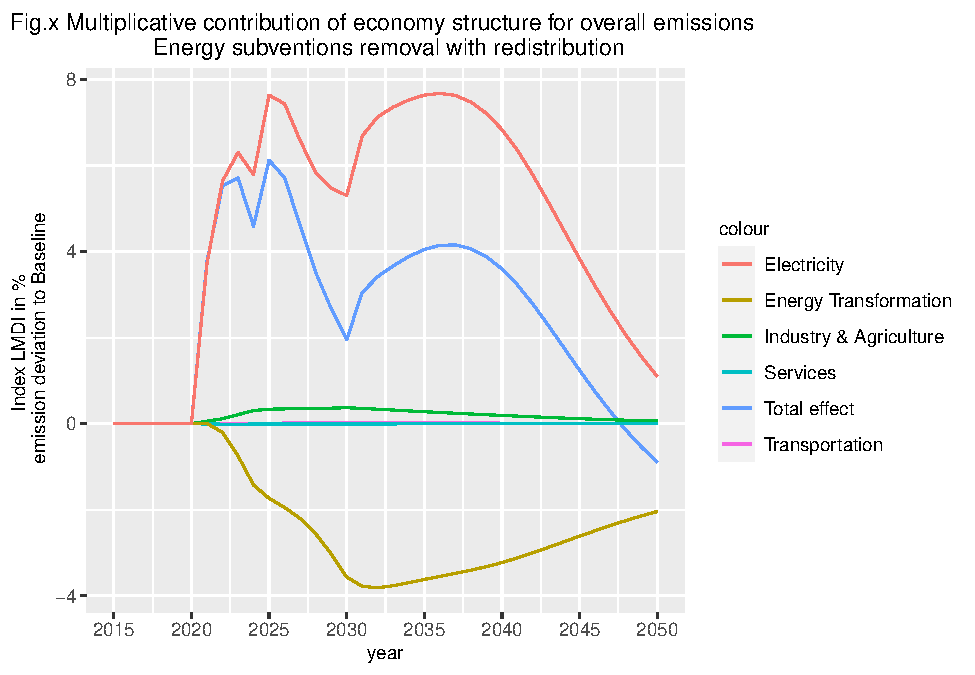
\includegraphics{02-01---Projet-Modélisation-Prospective-ThreeME_files/figure-latex/unnamed-chunk-30-1.pdf}

\begin{Shaded}
\begin{Highlighting}[]
\FunctionTok{ggplot}\NormalTok{() }\SpecialCharTok{+} 
  \FunctionTok{geom\_line}\NormalTok{( }\FunctionTok{aes}\NormalTok{(}\AttributeTok{x =}\NormalTok{ Det[[}\DecValTok{5}\NormalTok{]][,}\StringTok{"year"}\NormalTok{],}\AttributeTok{y =}\NormalTok{ Det[[}\DecValTok{6}\NormalTok{]][,}\StringTok{"I"}\NormalTok{], }\AttributeTok{group =} \DecValTok{1}\NormalTok{, }\AttributeTok{color =} \StringTok{"Effect Total"}\NormalTok{)) }\SpecialCharTok{+} 
  \FunctionTok{geom\_line}\NormalTok{( }\FunctionTok{aes}\NormalTok{(}\AttributeTok{x =}\NormalTok{ Det[[}\DecValTok{5}\NormalTok{]][,}\StringTok{"year"}\NormalTok{],}\AttributeTok{y =}\NormalTok{ Det[[}\DecValTok{6}\NormalTok{]][,}\StringTok{"I\_ind"}\NormalTok{], }\AttributeTok{group =} \DecValTok{1}\NormalTok{, }\AttributeTok{color =} \StringTok{"Industrie \& Agriculture"}\NormalTok{)) }\SpecialCharTok{+} 
  \FunctionTok{geom\_line}\NormalTok{( }\FunctionTok{aes}\NormalTok{(}\AttributeTok{x =}\NormalTok{ Det[[}\DecValTok{5}\NormalTok{]][,}\StringTok{"year"}\NormalTok{],}\AttributeTok{y =}\NormalTok{ Det[[}\DecValTok{6}\NormalTok{]][,}\StringTok{"I\_trsp"}\NormalTok{], }\AttributeTok{group =} \DecValTok{1}\NormalTok{, }\AttributeTok{color =} \StringTok{"Transport"}\NormalTok{)) }\SpecialCharTok{+} 
  \FunctionTok{geom\_line}\NormalTok{( }\FunctionTok{aes}\NormalTok{(}\AttributeTok{x =}\NormalTok{ Det[[}\DecValTok{5}\NormalTok{]][,}\StringTok{"year"}\NormalTok{],}\AttributeTok{y =}\NormalTok{ Det[[}\DecValTok{6}\NormalTok{]][,}\StringTok{"I\_ser"}\NormalTok{], }\AttributeTok{group =} \DecValTok{1}\NormalTok{, }\AttributeTok{color =} \StringTok{"Service"}\NormalTok{)) }\SpecialCharTok{+} 
  \FunctionTok{geom\_line}\NormalTok{( }\FunctionTok{aes}\NormalTok{(}\AttributeTok{x =}\NormalTok{ Det[[}\DecValTok{5}\NormalTok{]][,}\StringTok{"year"}\NormalTok{],}\AttributeTok{y =}\NormalTok{ Det[[}\DecValTok{6}\NormalTok{]][,}\StringTok{"I\_trsf"}\NormalTok{], }\AttributeTok{group =} \DecValTok{1}\NormalTok{, }\AttributeTok{color =} \StringTok{"Transformation énergétique"}\NormalTok{)) }\SpecialCharTok{+} 
  \FunctionTok{geom\_line}\NormalTok{( }\FunctionTok{aes}\NormalTok{(}\AttributeTok{x =}\NormalTok{ Det[[}\DecValTok{5}\NormalTok{]][,}\StringTok{"year"}\NormalTok{],}\AttributeTok{y =}\NormalTok{ Det[[}\DecValTok{6}\NormalTok{]][,}\StringTok{"I\_ele"}\NormalTok{], }\AttributeTok{group =} \DecValTok{1}\NormalTok{, }\AttributeTok{color =} \StringTok{"Electricité"}\NormalTok{)) }\SpecialCharTok{+}
  \FunctionTok{labs}\NormalTok{(}\AttributeTok{x =} \StringTok{"year"}\NormalTok{, }\AttributeTok{y =} \StringTok{"Variation d\textquotesingle{}émission CO2"}\NormalTok{, }\AttributeTok{title =} \StringTok{"Contribution multiplicative sur l\textquotesingle{}Intensité énergétique {-} Melange politique"}\NormalTok{) }\SpecialCharTok{+} 
  \FunctionTok{scale\_x\_continuous}\NormalTok{(}\AttributeTok{breaks=}\FunctionTok{seq}\NormalTok{(}\DecValTok{2015}\NormalTok{,}\DecValTok{2050}\NormalTok{,}\DecValTok{5}\NormalTok{))}
\end{Highlighting}
\end{Shaded}

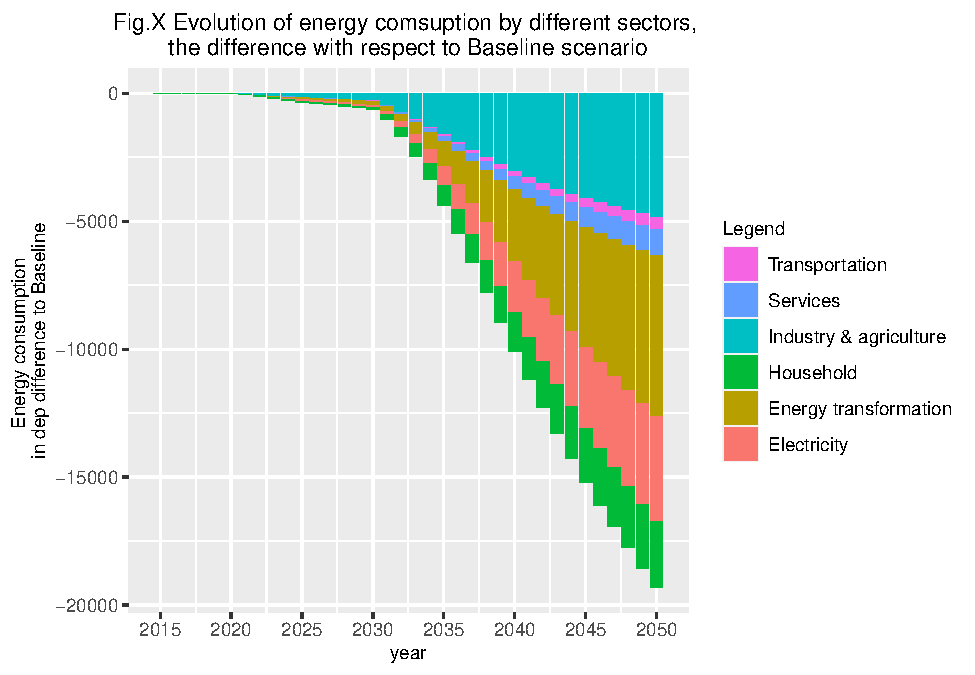
\includegraphics{02-01---Projet-Modélisation-Prospective-ThreeME_files/figure-latex/unnamed-chunk-31-1.pdf}

\begin{Shaded}
\begin{Highlighting}[]
\FunctionTok{ggplot}\NormalTok{() }\SpecialCharTok{+} 
  \FunctionTok{geom\_line}\NormalTok{( }\FunctionTok{aes}\NormalTok{(}\AttributeTok{x =}\NormalTok{ Det[[}\DecValTok{5}\NormalTok{]][,}\StringTok{"year"}\NormalTok{],}\AttributeTok{y =}\NormalTok{ Det[[}\DecValTok{6}\NormalTok{]][,}\StringTok{"U"}\NormalTok{], }\AttributeTok{group =} \DecValTok{1}\NormalTok{, }\AttributeTok{color =} \StringTok{"Effect Total"}\NormalTok{)) }\SpecialCharTok{+} 
  \FunctionTok{geom\_line}\NormalTok{( }\FunctionTok{aes}\NormalTok{(}\AttributeTok{x =}\NormalTok{ Det[[}\DecValTok{5}\NormalTok{]][,}\StringTok{"year"}\NormalTok{],}\AttributeTok{y =}\NormalTok{ Det[[}\DecValTok{6}\NormalTok{]][,}\StringTok{"U\_ind"}\NormalTok{], }\AttributeTok{group =} \DecValTok{1}\NormalTok{, }\AttributeTok{color =} \StringTok{"Industrie \& Agriculture"}\NormalTok{)) }\SpecialCharTok{+} 
  \FunctionTok{geom\_line}\NormalTok{( }\FunctionTok{aes}\NormalTok{(}\AttributeTok{x =}\NormalTok{ Det[[}\DecValTok{5}\NormalTok{]][,}\StringTok{"year"}\NormalTok{],}\AttributeTok{y =}\NormalTok{ Det[[}\DecValTok{6}\NormalTok{]][,}\StringTok{"U\_trsp"}\NormalTok{], }\AttributeTok{group =} \DecValTok{1}\NormalTok{, }\AttributeTok{color =} \StringTok{"Transport"}\NormalTok{)) }\SpecialCharTok{+} 
  \FunctionTok{geom\_line}\NormalTok{( }\FunctionTok{aes}\NormalTok{(}\AttributeTok{x =}\NormalTok{ Det[[}\DecValTok{5}\NormalTok{]][,}\StringTok{"year"}\NormalTok{],}\AttributeTok{y =}\NormalTok{ Det[[}\DecValTok{6}\NormalTok{]][,}\StringTok{"U\_ser"}\NormalTok{], }\AttributeTok{group =} \DecValTok{1}\NormalTok{, }\AttributeTok{color =} \StringTok{"Service"}\NormalTok{)) }\SpecialCharTok{+} 
  \FunctionTok{geom\_line}\NormalTok{( }\FunctionTok{aes}\NormalTok{(}\AttributeTok{x =}\NormalTok{ Det[[}\DecValTok{5}\NormalTok{]][,}\StringTok{"year"}\NormalTok{],}\AttributeTok{y =}\NormalTok{ Det[[}\DecValTok{6}\NormalTok{]][,}\StringTok{"U\_trsf"}\NormalTok{], }\AttributeTok{group =} \DecValTok{1}\NormalTok{, }\AttributeTok{color =} \StringTok{"Transformation énergétique"}\NormalTok{)) }\SpecialCharTok{+} 
  \FunctionTok{geom\_line}\NormalTok{( }\FunctionTok{aes}\NormalTok{(}\AttributeTok{x =}\NormalTok{ Det[[}\DecValTok{5}\NormalTok{]][,}\StringTok{"year"}\NormalTok{],}\AttributeTok{y =}\NormalTok{ Det[[}\DecValTok{6}\NormalTok{]][,}\StringTok{"U\_ele"}\NormalTok{], }\AttributeTok{group =} \DecValTok{1}\NormalTok{, }\AttributeTok{color =} \StringTok{"Electricité"}\NormalTok{)) }\SpecialCharTok{+}
  \FunctionTok{labs}\NormalTok{(}\AttributeTok{x =} \StringTok{"year"}\NormalTok{, }\AttributeTok{y =} \StringTok{"Variation d\textquotesingle{}émission CO2"}\NormalTok{, }\AttributeTok{title =} \StringTok{"Contribution multiplicative sur l\textquotesingle{}Intensité carbone {-} Melange politique"}\NormalTok{) }\SpecialCharTok{+} 
  \FunctionTok{scale\_x\_continuous}\NormalTok{(}\AttributeTok{breaks=}\FunctionTok{seq}\NormalTok{(}\DecValTok{2015}\NormalTok{,}\DecValTok{2050}\NormalTok{,}\DecValTok{5}\NormalTok{))}
\end{Highlighting}
\end{Shaded}

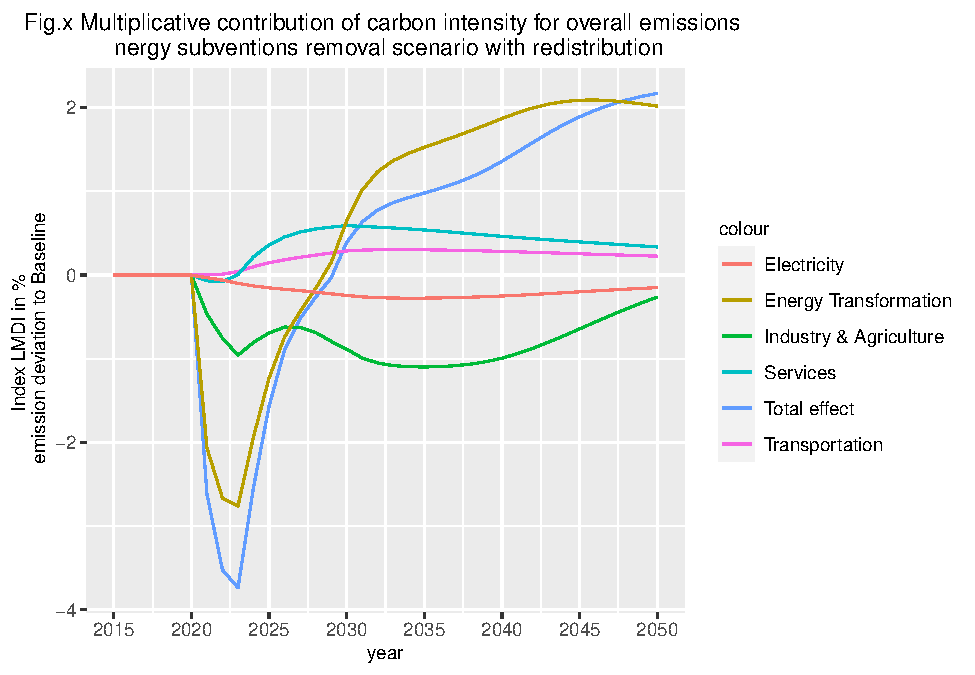
\includegraphics{02-01---Projet-Modélisation-Prospective-ThreeME_files/figure-latex/unnamed-chunk-32-1.pdf}

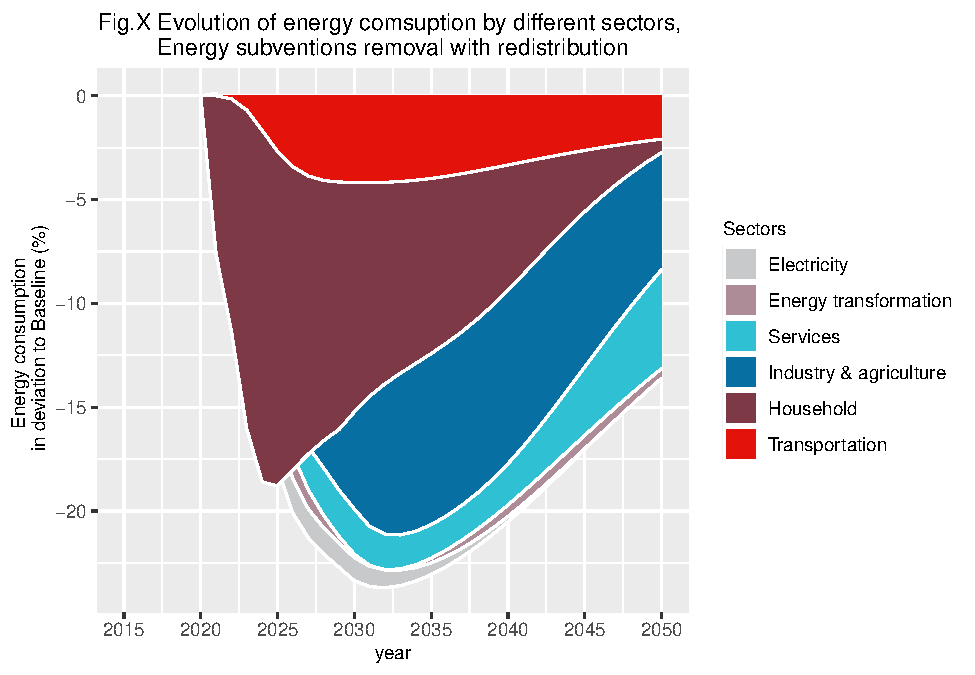
\includegraphics{02-01---Projet-Modélisation-Prospective-ThreeME_files/figure-latex/unnamed-chunk-33-1.pdf}

\hypertarget{iv.-economie}{%
\section{IV. Economie}\label{iv.-economie}}

\hypertarget{a.-production}{%
\subsection{A. Production}\label{a.-production}}

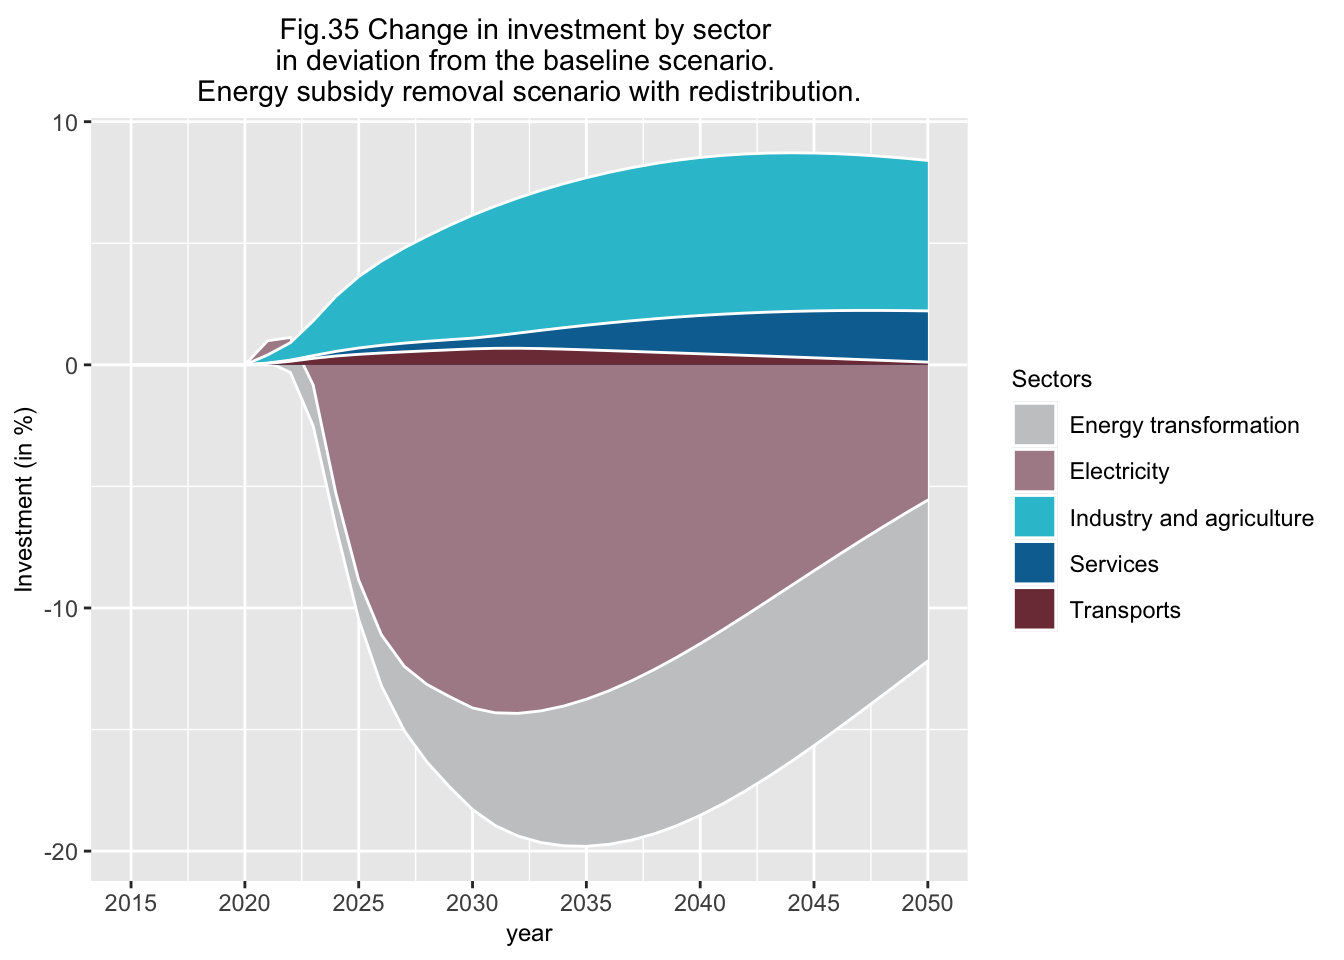
\includegraphics{02-01---Projet-Modélisation-Prospective-ThreeME_files/figure-latex/unnamed-chunk-34-1.pdf}

\hypertarget{c.-prix}{%
\subsection{C. Prix}\label{c.-prix}}

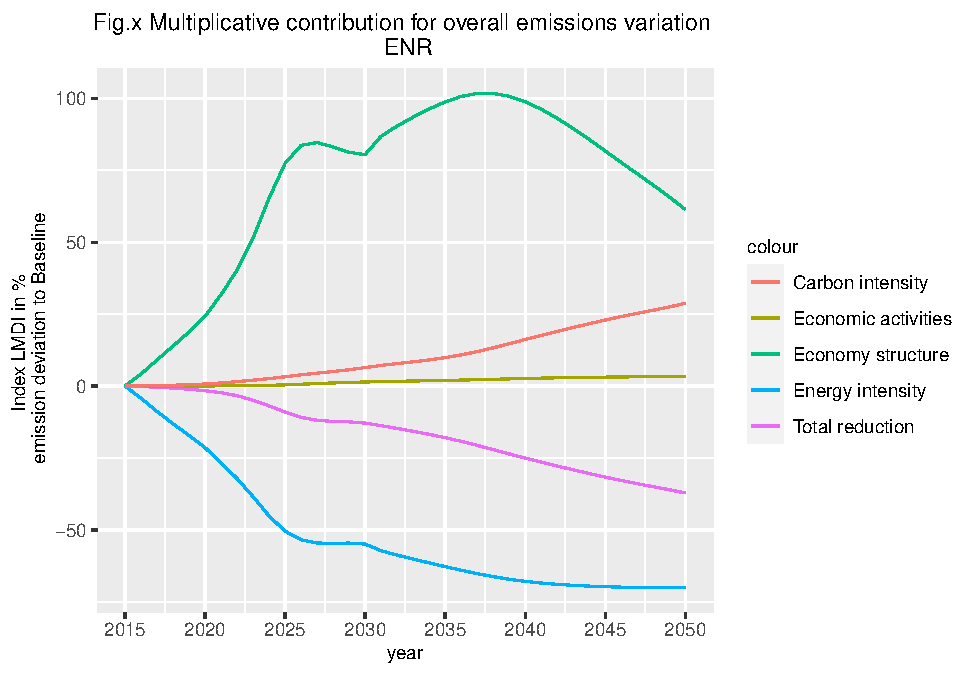
\includegraphics{02-01---Projet-Modélisation-Prospective-ThreeME_files/figure-latex/unnamed-chunk-35-1.pdf}

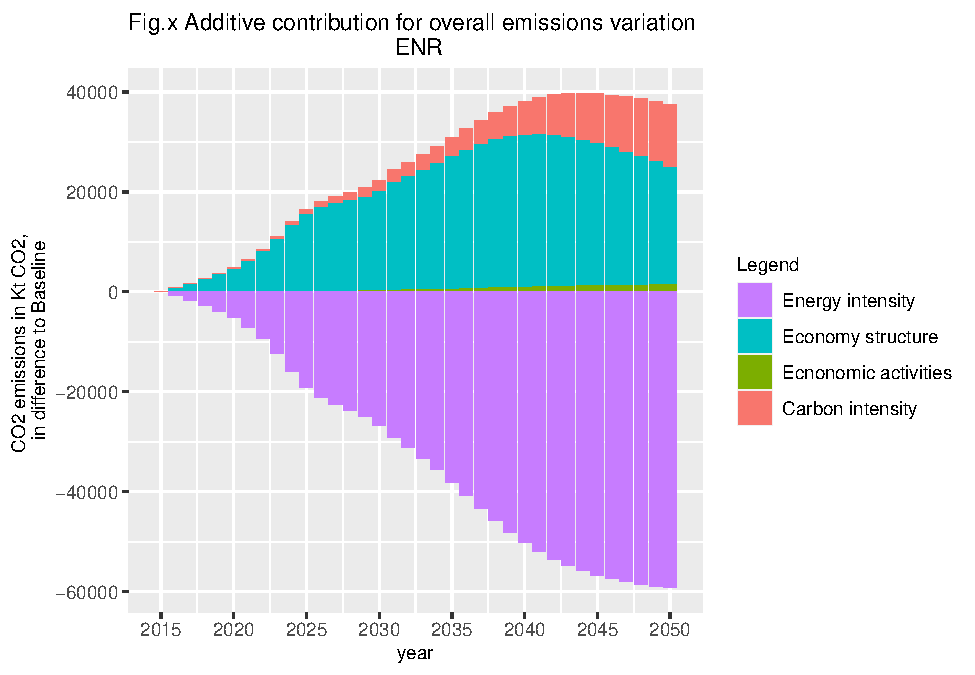
\includegraphics{02-01---Projet-Modélisation-Prospective-ThreeME_files/figure-latex/unnamed-chunk-36-1.pdf}

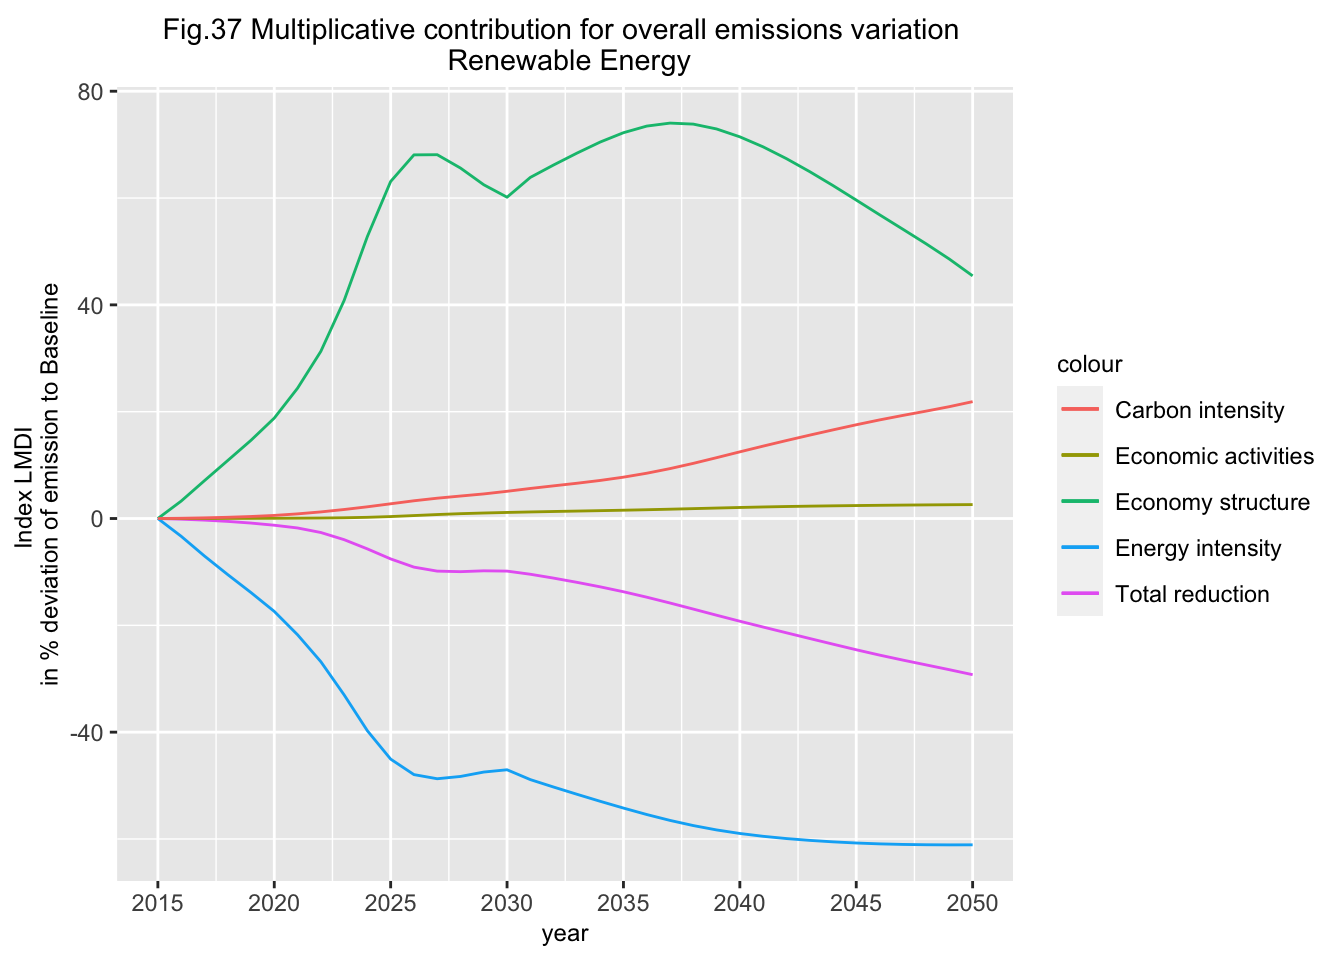
\includegraphics{02-01---Projet-Modélisation-Prospective-ThreeME_files/figure-latex/unnamed-chunk-37-1.pdf}

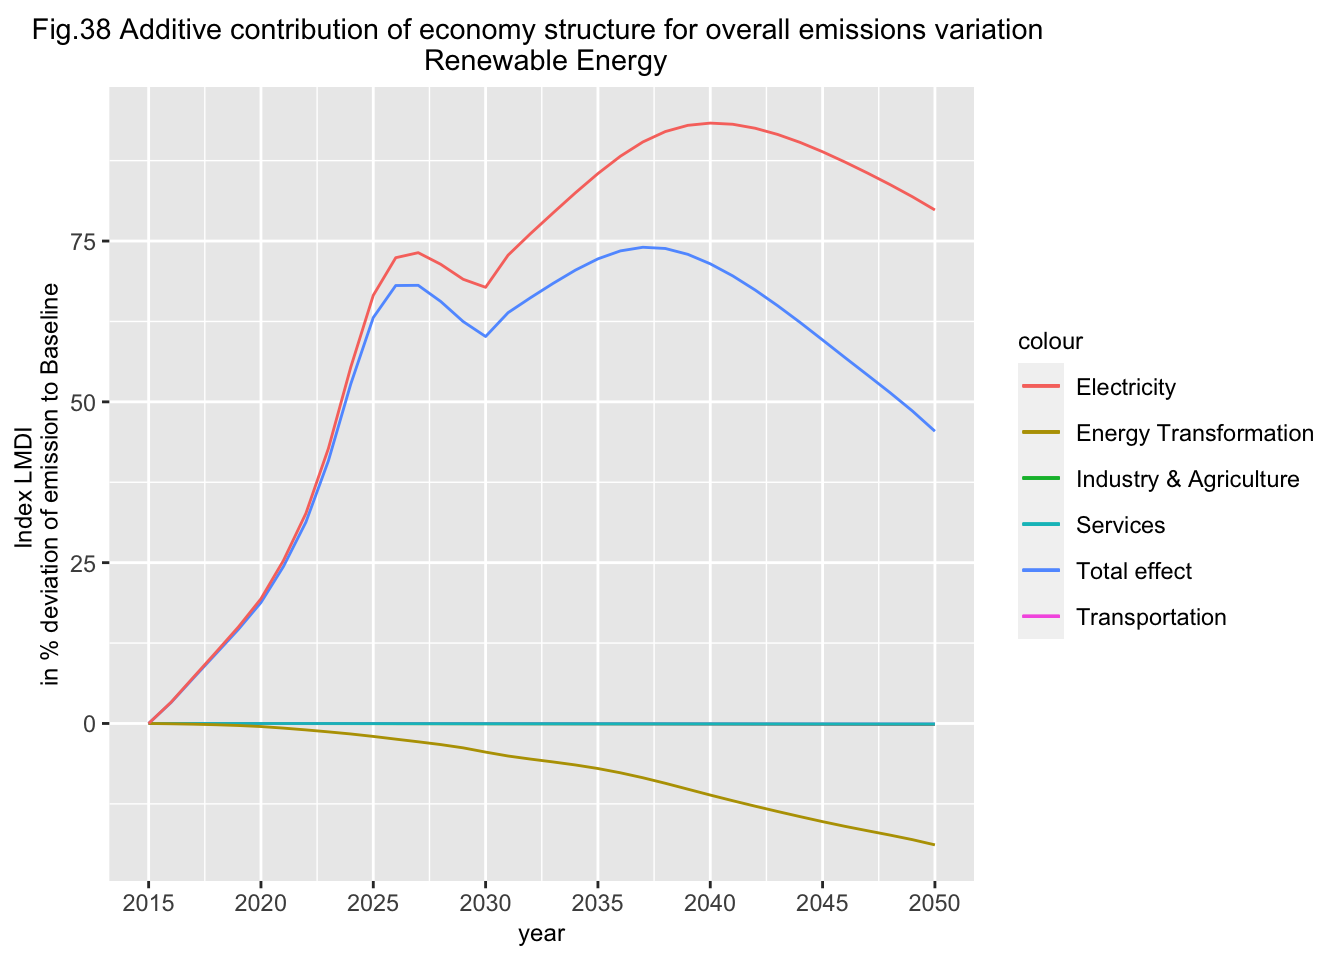
\includegraphics{02-01---Projet-Modélisation-Prospective-ThreeME_files/figure-latex/unnamed-chunk-38-1.pdf}

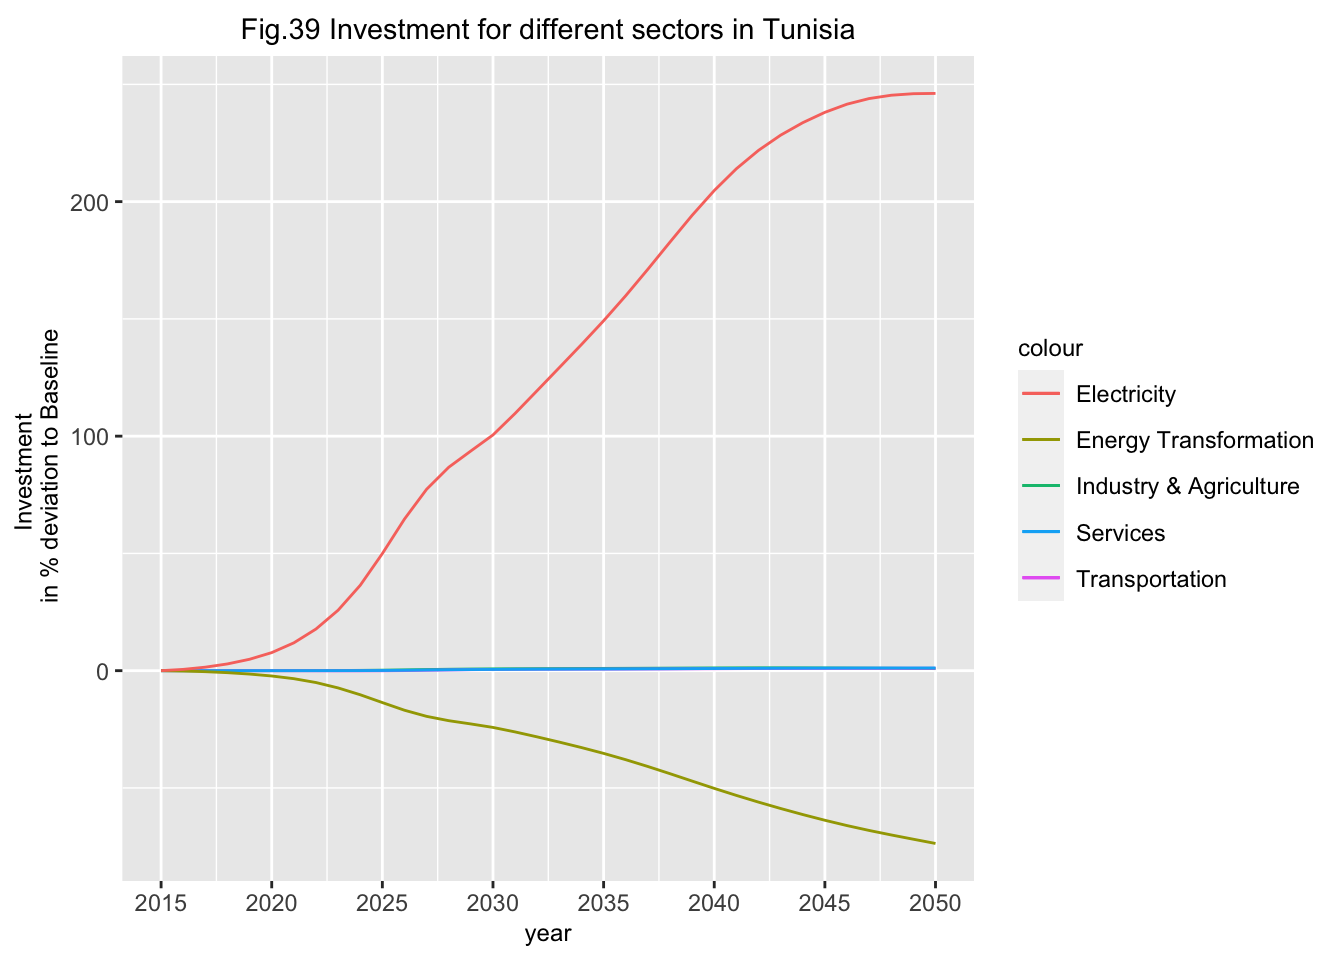
\includegraphics{02-01---Projet-Modélisation-Prospective-ThreeME_files/figure-latex/unnamed-chunk-39-1.pdf}

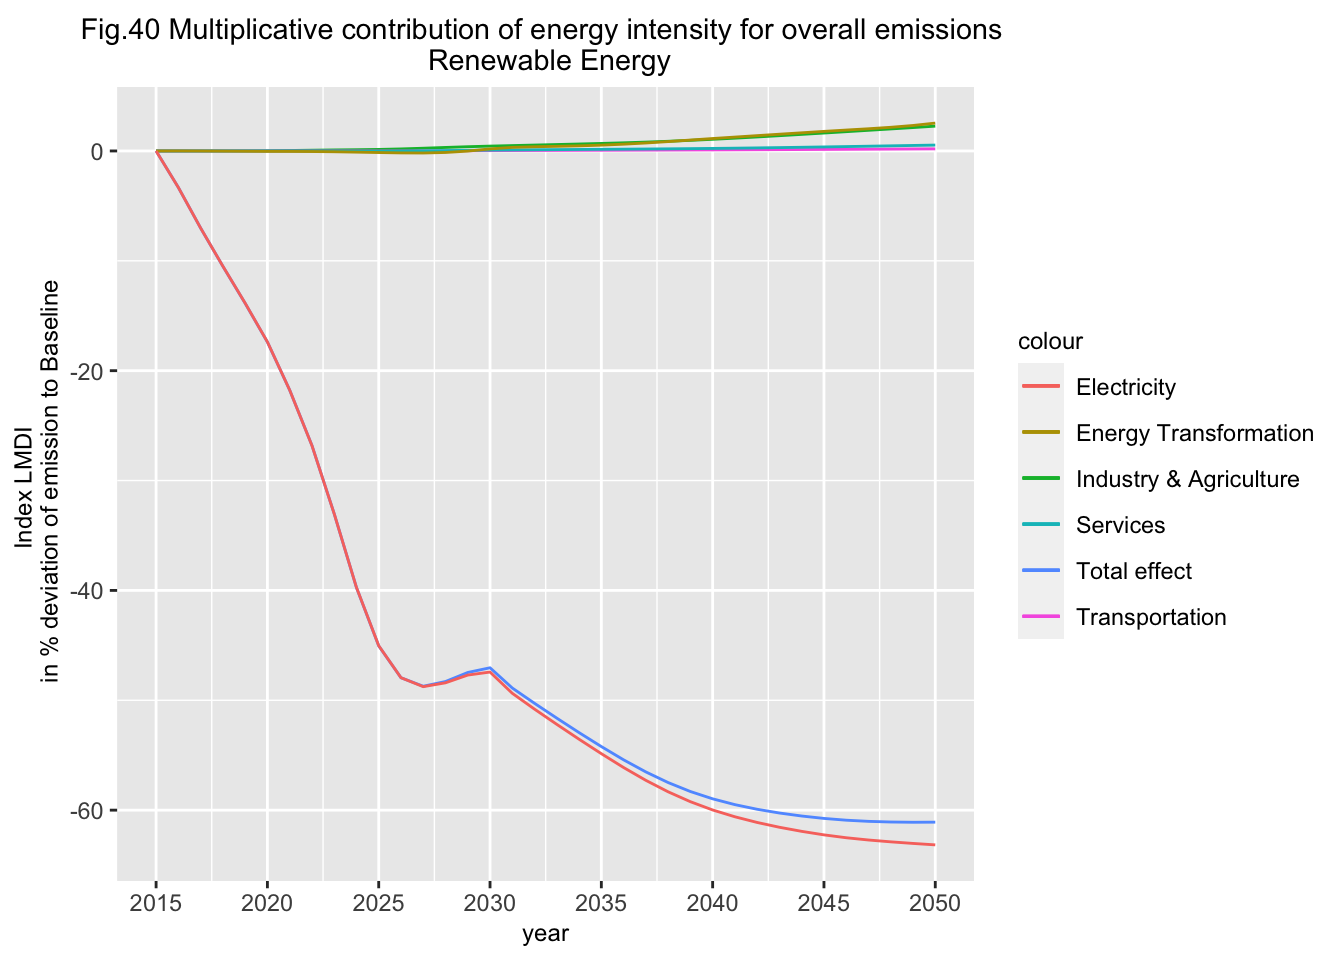
\includegraphics{02-01---Projet-Modélisation-Prospective-ThreeME_files/figure-latex/unnamed-chunk-40-1.pdf}

\hypertarget{c.-politiques-publiques---taxe-carbone-et-levuxe9e-des-subventions}{%
\subsection{C. Politiques publiques - Taxe carbone et levée des
subventions}\label{c.-politiques-publiques---taxe-carbone-et-levuxe9e-des-subventions}}

\includegraphics{02-01---Projet-Modélisation-Prospective-ThreeME_files/figure-latex/unnamed-chunk-41-1.pdf}

\includegraphics{02-01---Projet-Modélisation-Prospective-ThreeME_files/figure-latex/unnamed-chunk-42-1.pdf}

\hypertarget{d.-commerce-extuxe9rieur}{%
\subsection{D. Commerce extérieur}\label{d.-commerce-extuxe9rieur}}

\includegraphics{02-01---Projet-Modélisation-Prospective-ThreeME_files/figure-latex/unnamed-chunk-43-1.pdf}

\hypertarget{e.-emploi---report-shock}{%
\subsection{E. Emploi - Report shock}\label{e.-emploi---report-shock}}

\hypertarget{emploi-interscuxe9nario---niveau-agruxe9guxe9}{%
\subsubsection{1. Emploi interscénario - Niveau
agrégé}\label{emploi-interscuxe9nario---niveau-agruxe9guxe9}}

\includegraphics{02-01---Projet-Modélisation-Prospective-ThreeME_files/figure-latex/unnamed-chunk-44-1.pdf}

\includegraphics{02-01---Projet-Modélisation-Prospective-ThreeME_files/figure-latex/unnamed-chunk-45-1.pdf}

\includegraphics{02-01---Projet-Modélisation-Prospective-ThreeME_files/figure-latex/unnamed-chunk-46-1.pdf}

\begin{Shaded}
\begin{Highlighting}[]
\NormalTok{create\_beautiful\_radarchart }\OtherTok{\textless{}{-}} \ControlFlowTok{function}\NormalTok{(data, }\AttributeTok{color =} \StringTok{"\#00AFBB"}\NormalTok{, }
                                        \AttributeTok{vlabels =} \FunctionTok{colnames}\NormalTok{(data), }\AttributeTok{vlcex =} \FloatTok{0.7}\NormalTok{,}
                                        \AttributeTok{caxislabels =} \ConstantTok{NULL}\NormalTok{, }\AttributeTok{title =} \ConstantTok{NULL}\NormalTok{, ...)\{}
  \FunctionTok{radarchart}\NormalTok{(}
\NormalTok{    data, }\AttributeTok{axistype =} \DecValTok{1}\NormalTok{,}
    \CommentTok{\# Personnaliser le polygone}
    \AttributeTok{pcol =}\NormalTok{ color, }\AttributeTok{pfcol =}\NormalTok{ scales}\SpecialCharTok{::}\FunctionTok{alpha}\NormalTok{(color, }\FloatTok{0.5}\NormalTok{), }\AttributeTok{plwd =} \DecValTok{2}\NormalTok{, }\AttributeTok{plty =} \DecValTok{1}\NormalTok{,}
    \CommentTok{\# Personnaliser la grille}
    \AttributeTok{cglcol =} \StringTok{"grey"}\NormalTok{, }\AttributeTok{cglty =} \DecValTok{1}\NormalTok{, }\AttributeTok{cglwd =} \FloatTok{0.8}\NormalTok{,}
    \CommentTok{\# Personnaliser l\textquotesingle{}axe}
    \AttributeTok{axislabcol =} \StringTok{"grey"}\NormalTok{, }
    \CommentTok{\# Étiquettes des variables}
    \AttributeTok{vlcex =}\NormalTok{ vlcex, }\AttributeTok{vlabels =}\NormalTok{ vlabels,}
    \AttributeTok{caxislabels =}\NormalTok{ caxislabels, }\AttributeTok{title =}\NormalTok{ title, ...}
\NormalTok{  )}
\NormalTok{\}}
\end{Highlighting}
\end{Shaded}

\begin{Shaded}
\begin{Highlighting}[]
\FunctionTok{library}\NormalTok{(fmsb)}


\NormalTok{data\_radar }\OtherTok{\textless{}{-}}\NormalTok{deltaf\_l[}\DecValTok{36}\NormalTok{,}\FunctionTok{c}\NormalTok{(}\DecValTok{2}\SpecialCharTok{:}\DecValTok{7}\NormalTok{)]}



\FunctionTok{colnames}\NormalTok{(data\_radar)}\OtherTok{\textless{}{-}}\FunctionTok{c}\NormalTok{(}\StringTok{"Taxe sans redistribution"}\NormalTok{,}\StringTok{"Taxe avec redistribution"}\NormalTok{,}\StringTok{"Subvention sans redistribution"}\NormalTok{,}\StringTok{"Taxe avec redistribution"}\NormalTok{,}\StringTok{"ENR"}\NormalTok{,}\StringTok{"SNBC"}\NormalTok{)}

\NormalTok{data\_radar  }\OtherTok{=} \FunctionTok{as.data.frame}\NormalTok{(data\_radar)}
\NormalTok{data\_radar  }\OtherTok{=} \FunctionTok{rbind}\NormalTok{(}\DecValTok{225}\NormalTok{,}\SpecialCharTok{{-}}\DecValTok{50}\NormalTok{, }\DecValTok{0}\NormalTok{, data\_radar)}





\NormalTok{op }\OtherTok{\textless{}{-}} \FunctionTok{par}\NormalTok{(}\AttributeTok{mar =} \FunctionTok{c}\NormalTok{(}\DecValTok{1}\NormalTok{, }\DecValTok{2}\NormalTok{, }\DecValTok{2}\NormalTok{, }\DecValTok{1}\NormalTok{), }\AttributeTok{cex.main=}\FloatTok{0.9}\NormalTok{)}
\FunctionTok{create\_beautiful\_radarchart}\NormalTok{(data\_radar, }\AttributeTok{caxislabels =} \FunctionTok{c}\NormalTok{(}\SpecialCharTok{{-}}\DecValTok{50}\NormalTok{, }\DecValTok{0}\NormalTok{, }\DecValTok{100}\NormalTok{,}\DecValTok{150}\NormalTok{,}\DecValTok{200}\NormalTok{,}\DecValTok{250}\NormalTok{), }\AttributeTok{color =} \FunctionTok{c}\NormalTok{(}\ConstantTok{NA}\NormalTok{,}\StringTok{"\#00AFBB"}\NormalTok{), }\AttributeTok{title=}\StringTok{"Variation d\textquotesingle{}emploi en 2050. }
\StringTok{Ecart par rapport au scénario en référence (en milliers d\textquotesingle{}emploi)."}\NormalTok{)}
\end{Highlighting}
\end{Shaded}

\includegraphics{02-01---Projet-Modélisation-Prospective-ThreeME_files/figure-latex/CREATION GRAPHIQUE RADAR-1.pdf}

\begin{Shaded}
\begin{Highlighting}[]
\FunctionTok{par}\NormalTok{(op)}
\end{Highlighting}
\end{Shaded}

\hypertarget{emploi-par-scuxe9nario---niveau-sectoriel}{%
\subsubsection{2. Emploi par scénario - Niveau
sectoriel}\label{emploi-par-scuxe9nario---niveau-sectoriel}}

Peu concluant, pas beaucoup de variation (même en relatif) à part pour
la transformation d'énergie (voir peut-être les missing data pour avoir
plus de secteurs)

\includegraphics{02-01---Projet-Modélisation-Prospective-ThreeME_files/figure-latex/unnamed-chunk-47-1.pdf}

\includegraphics{02-01---Projet-Modélisation-Prospective-ThreeME_files/figure-latex/unnamed-chunk-48-1.pdf}

\includegraphics{02-01---Projet-Modélisation-Prospective-ThreeME_files/figure-latex/unnamed-chunk-49-1.pdf}

\includegraphics{02-01---Projet-Modélisation-Prospective-ThreeME_files/figure-latex/unnamed-chunk-50-1.pdf}

\end{document}
